\documentclass{template/abschlussarbeit}

%%%%%%%%%%%%%%%%%%%%%%%%%%%%%%%%%%%%%%%%%%%%%%%%%%%%%%%%%%%%
% Allgemeine Variablen fuer die Abschlussarbeit (mit eigenen
% Angaben ausfuellen!)
%%%%%%%%%%%%%%%%%%%%%%%%%%%%%%%%%%%%%%%%%%%%%%%%%%%%%%%%%%%%

\AutorVorname{Nils}
\AutorNachname{Axer}
\AutorGeburtsort{Gräfelfing}
\AbschlussarbeitTitel{Ein streng konsistenter Koordinierungsdienst als Basis für verteilte Anwendungen}
% Bachelorarbeit, Projektarbeit, Masterarbeit
\AbschlussarbeitTyp{Masterarbeit}
% keywords durch , getrennt
\AbschlussarbeitKeywords{Distributed Systems, Big Data, Cloud}
\Ort{Düsseldorf}
\Datum{2. Mai 2019}
\Erstgutachter{Prof. Dr. Michael Schöttner}
\Zweitgutachter{Prof. Dr. Martin Mauve}
\Betreuer{Stefan Nothaas}

% Hier den vollstaendigen Dateinamen der bibtex Datei angeben
% Falls diese in einem Unterordner liegt, so ist dieser relativ
% zu dieser Datei (document.tex) anzugeben.
\LiteraturBibtexDatei{library}

% Der Anhang (falls vorhanden) wird hier genauso wie diese
% Bibtex-Datei angegeben (jedoch ohne .tex-Endung!)
\AnhangDatei{chap/anhang}

%%%%%%%%%%%%%%%%%%%%%%%%%%%%%%%%%%%%%%%%%%%%%%%%%%%%%%%%%%%%
% Optionen/Schalter um bestimmte Abschnitte an-/auszuschalten
% WICHTIG: Nicht genutzte/leere Abschnitte vor der Abgabe/
% dem finalen Druck abschalten durch auskommentieren.
% Gleiches gilt fuer die Todo Liste, welche nicht in die 
% finale Version gehoert.
%%%%%%%%%%%%%%%%%%%%%%%%%%%%%%%%%%%%%%%%%%%%%%%%%%%%%%%%%%%%

\Titelblatt
\TodoListe
\Inhaltsverzeichnis
\Abbildungsverzeichnis
\Tabellenverzeichnis
\Algorithmenverzeichnis
\Anhang
\Erklaerung

%%%%%%%%%%%%%%%%%%%%%%%%%%%%%%%%%%%%%%%%%%%%%%%%%%%%%%%%%%%%

\begin{document}
\begin{abschlussarbeit}

%%%%%%%%%%%%%%%%%%%%%%%%%%%%%%%%%%%%

% Hier werden die einzelnen Kapitel aufgelistet (Reihenfolge!)
% Die vorgegebenen Kapitel dienen als Hilfestellung waehrend der Arbeit
% und sind mit der Fertigstellung des finalen Dokuments zu entfernen!
\chapter{Einleitung}

\section{Motivation}

\section{Anforderungen}

\section{Ziele der Arbeit}
\label{ziele}

\chapter{Theorie}
\label{theory}

\section{CAP-Theorem}
\label{cap}

Um ein System zu entwerfen, das die Anforderungen erfüllt, ist es zunächst wichtig herauszufinden, welche Eigenschaften ein verteiltes System überhaupt theoretisch erfüllen kann. Dabei hilft das CAP-Theorem \cite{cap}. Es beweist, dass ein verteilter Speicher von den drei Eigenschaften 
\begin{itemize}
	\item \textbf{Konsistenz}: Wird von den Autoren als \textit{Linearizability} (auch \textit{Atomic Consistency}) definiert: Wenn ein Write abgeschlossen ist, müssen alle Reads, die danach beginnen, den Wert des Writes oder eines späteren Writes zurückgeben. Dies ist ein sehr starkes Konsistenzmodell.
	\item \textbf{Verfügbarkeit}: Das System ist zu jedem Zeitpunkt erreichbar und antwortet auf alle Anfragen an nicht abgestürzte Knoten.
	\item \textbf{Partitionstoleranz}: Das System funktioniert weiter falls das Netzwerk partitioniert wird, also ein Teil der Knoten von einem anderen Teil abgeschnitten ist.
\end{itemize}
 höchstens zwei gleichzeitig erfüllen kann. 

Konsistenz und Verfügbarkeit kann man als graduelle Eigenschaften ansehen. Im CAP-Theorem wird von einem sehr starken Konsistenzmodell ausgegangen, das sich je nach Anwendung auch lockern lässt. Ebenso kann man die Verfügbarkeit graduell anpassen. Es muss also abgewogen werden, welche dieser Eigenschaften für ein System wichtig sind und welche nicht. Deshalb kann es viele verschiedene System mit verschiedenen Eigenschaften für ganz unterschiedliche Einsatzgebiete geben. Partitionstoleranz ist in der Realtität wichtig, da man diese in typischen Einsatzorten wie Datenzentren nie ausschließen kann. Netzwerkpartitionierungen können z.B. durch Ausfälle von einzelnen Switches oder Routern hervorgerufen werden. 

Sehr viele verteilte Systeme sind auf hohe Verfügbarkeit optimiert, da sie z.B. ständig über das Internet erreichbar sein sollen. Darunter sind z.B. die meisten SQL- und NoSQL-Datenbanken und Key-Value-Stores wie DXRAM. SQL-Datenbanken wollen nach dem ACID-Prinzip möglich starke Konsistenz der Daten, weshalb sie meist die Partitionstoleranz aufgeben. NoSQL-Datenbanken lockern das Konsistenzmodell nach dem BASE-Prinzip und versuchen dadurch die Partitionstoleranz zu erreichen. Einige Systeme verwenden auch ein externes System um wichtige Daten, die auch bei einer Netzwerkpartitionierung noch konsistent vorhanden sein müssen, separat zu speichern. Dies ist ein Anwendungsgebiet für das System, das in dieser Arbeit entworfen werden soll.

Ein weiteres Beispiel für ein System, welches die Konsistenz zugunsten der Verfügbarkeit und der Partitionstoleranz abschwächt, ist das Domain Name System (DNS). Die DNS-Einträge werden auf den Nameservern für eine bestimmte Zeit zwischengespeichert, um Verfügbarkeit und Partitionstoleranz zu erreichen. Dadurch ist es jedoch möglich, dass diese Caches nicht aktuell und somit nicht konsistent zu ihren Ursprüngen sind.

Besonders wichtig für das System, das in dieser Arbeit entworfen werden soll, ist die Konsistenz. Alle Knoten im verteilten System sollten stets die gleiche Sicht auf den Status haben, sodass sie sich koordinieren und auf bestimmte Dinge einigen können. Dafür muss gerade die \textit{Atomic Consistency} erreicht werden, die auch im CAP-Theorem verwendet wird.

Um Konsistenz in einem verteilten System zu erreichen, muss das fundamentale Problem der Einigung auf einen Wert (oder einer Sequenz von Werten) gelöst werden. Wenn sich alle Knoten eines verteilten Systems auf den gleichen Wert geeinigt haben und dieser für alle sichtbar ist, dann ist das System für alle Knoten konsistent. Algorithmen, die dies ermöglichen, nennt man deshalb \textit{Einigungsalgorithmen}.

Da das Problem im Allgemeinen nicht trivial ist, sollen im Folgenden ein paar Algorithmen vorgestellt werden, die das Problem mit vereinfachten Modellen, die meist nicht den realen Bedingungen entsprechen, lösen.

\subsection{Flooding Consensus}

Der Flooding Consensus Algorithmus löst das Einigungsproblem in einem synchronen System und mit einem Fail-Stop-Modell, d.h. Server können abstürzen und senden dann keine Nachrichten mehr. Der Algorithmus läuft in \textit{n} Runden ab. Jeder Server hat zu Beginn einen Wert und speichert sich die gesamte Liste der empfangenen Werte. In jeder Runde flutet jeder Server das Netzwerk mit seinen bekannten Werten, d.h. er sendet seine Liste an alle teilnehmenden Server. Falls in einer Runde mindestens ein Server beim Senden oder vor dem Senden ausfällt, kann in dieser Runde keine Einigung erreicht werden, da es sein kann, dass die Server unterschiedliche Werte in ihren Listen haben. Um \textit{f} fehlerhafte Server zu kompensieren, werden also maximal \textit{f+1} Runden benötigt, bis die Server alle die gleichen Werte in ihren Listen haben. Dann können sie mit einer Funktion, die auf der Liste ausgeführt wird, den Entscheidungswert bestimmen. Dies könnte z.B. die Maximumsfunktion sein.
Um festzustellen, wann eine Runde vorbei ist, muss die maximale Nachrichtenlaufzeit und die maximale Bearbeitungszeit bekannt sein. Wenn dies bekannt ist, können die Server in jeder Runde diese Zeit abwarten und es ist sicher, dass ein Server, von dem in dieser Zeit keine Nachricht erhalten wurde, abgestürzt ist. Da man diese Zeit in der Praxis jedoch normalerweise nicht bestimmen kann, ist dieser Algorithmus meistens nicht für einen Einsatz geeignet.

\subsection{2-Phase-Commit}

Der 2-Phase-Commit-Algorithmus löst das Einigungsproblem in einem asynchronen System mit einer perfekten Ausfallerkennung. Hier geschieht die Einigung mithilfe eines Koordinators, der vorher mit einem externen Verfahren bestimmt werden muss, z.B. einem Leader-Election-Algorithmus. Da der Koordinator auch ausfallen kann und ein neuer Koordinator einen inkonsistenten Wert verbreiten könnte, kann dieser nicht einfach alle Werte einsammeln und entscheiden, sondern der Algorithmus muss in zwei Phasen durchgeführt werden:

\begin{itemize}
	\item \textbf{Phase 1}: Der Koordinator sendet eine \textit{propose}-Nachricht an alle Server mit seinem Wert, auf den sich geeinigt werden soll. Die Server akzeptieren den vorgeschlagenen Wert und merken sich diesen. Der Koordinator wartet auf Antworten von allen nicht ausgefallenen Servern (hier wird die Ausfallerkennung benötigt). Sobald er von allen Servern eine Antwort erhalten hat, ist es sicher, dass ein möglicher neuer Koordinator denselben Wert verbreiten wird, falls dieser Koordinator ausfällt. Die Aktivierung eines neuen Koordinators kann ebenfalls nur durch die perfekte Ausfallerkennung erreicht werden, sonst kann es sein, dass es mehrere oder keinen Koordinator gibt.
	\item \textbf{Phase 2}: Der Koordinator sendet eine \textit{decide}-Nachricht an alle Server, die die Entscheidung auf den vorgeschlagenen Wert darstellt. Sobald er von allen Server eine Antwort erhalten hat, haben sich alle Server auf diesen Wert geeinigt.
\end{itemize}

Der 2-Phase-Commit Algorithmus wird in der Praxis eingesetzt, z..B. in der Oracle Database \cite{oracle-db-2pc} um verteilte Transaktionen zu ermöglichen. Da es dabei jedoch keine perfekte Ausfallerkennung gibt, wird bei unerfolgreichem Ausführen des Algorithmus, z.B. bei Ausfällen oder Nachrichtenverlusten, die Datenbank blockiert und die Transaktion als \glqq In-Doubt \grqq markiert. Die Datenbank versucht dann, den Fehler automatisch zu beheben, dies kann jedoch nicht in allen Fällen geschehen. Dann muss der Fehler manuell behoben werden.

Da der Algorithmus keine Fehlertoleranz garantieren kann und blockiert, sobald einer der teilnehmenden Server ausfällt, ist er nicht für das System, das in dieser Arbeit entworfen werden soll, geeignet. 

\section{FLP-Theorem}

Zum Verständnis von Einigungsalgorithmen ist noch ein weiteres Theorem wichtig: Das FLP-Theorem \cite{flp}. Es zeigt, dass es keinen Einigungsalgorithmus in einem \textbf{asynchronen System} geben kann, der bei Knotenausfällen korrekt arbeitet und immer terminiert. Ähnlich wie bei CAP-Theorem kann man hier ebenfalls drei Eigenschaften formulieren, die ein Algorithmus nicht gleichzeitig erfüllen kann: Sicherheit, Verfügbarkeit und Fehlertoleranz. Ein Unterschied zum CAP-Theorem ist, dass hier von einem schwächeren Modell ausgegangen wird: Die teilnehmenden Server können zwar abstürzen, das Netzwerk ist jedoch zuverlässig und es kann insbesondere keine Netzwerkpartitionierung geben.
Alle Einigungsalgorithmen, die auf einem asynchronem Modell basieren, sind also nur partiell korrekt. Für die in dieser Arbeit vorgestellten Algorithmen bedeutet dies, dass sie sich auf die Eigenschaften Sicherheit und Fehlertoleranz fokussieren. Dadurch kann man im Allgemeinen nicht beweisen, dass sie auch terminieren. Meist wird durch geschickt gewählte Timeouts oder Ähnliches in der Praxis erreicht, dass die Algorithmen zur meisten Zeit terminieren und zu einem Ergebnis kommen.
Tatsächlich gibt es auch Einigungsalgorithmen, die immer terminieren, jedoch dafür die Sicherheit oder die Fehlertoleranz opfern. Beispiele für Algorithmen, bei denen es zugunsten der Terminierung manchmal falsche Ergebnisse geben kann, sind der 3-Phase-Commit-Algorithmus \cite{pc} und probabilistische Algorithmen wie Proof-of-Work in Blockchains \todo[inline]{genauer erklären}.


\section{Crash-Recovery-Modell}

Alle in dieser Arbeit vorgestellten Einigungsalgorithmen basieren auf dem \textit{Crash-Recovery-Modell}. Server arbeiten asynchron, können abstürzen und nach einem Neustart wieder am Cluster teilnehmen. Außerdem kann das Netzwerk unzuverlässig sein. Nachrichten können also beliebig viel Zeit von einem Knoten zu einem anderen Knoten benötigen, verloren gehen oder die Reihenfolge ändern. Ziel dabei ist, dass der Einigungsalgorithmus solange eine Einigung erzielen kann, wie eine Mehrheit der Server funktioniert und erreichbar ist. Die teilnehmenden Server dürfen sich jedoch nicht beliebig falsch verhalten, also keine falschen Nachrichten schicken und keine Systemzustände erreichen, die nicht vorgesehen sind. Es gibt auch Einigungsalgorithmen, die gegen solche byzantinischen Fehler geschützt sind \cite{byzantine-paxos}, jedoch erhöht dies die Komplexität deutlich und es werden im Vergleich zum Crash-Recovery-Modell mehr Server benötigt, um sich vor der gleichen Anzahl an fehlerhaften bzw. ausfallenden Servern zu schützen, was das System insgesamt langsamer macht.

\section{Einigungsalgorithmen}
\label{algos}

\subsection{Paxos}

Der bekannteste Einigungsalgorithmus ist Paxos \cite{paxos, paxos-made-simple}. Paxos implementiert eine \textit{Replicated State Machine}. \todo[inline]{Grafik zur Replicated State Machine} Bei diesem Modell besitzt jeder Knoten eine Zustandsmaschine, die Befehle ausführt und dadurch den Zustand ändert. Der Einigungsalgorithmus kümmert sich darum, dass die Befehle auf allen Knoten in der gleichen Reihenfolge durchgeführt werden, sodass der Zustand auf allen Knoten konsistent ist.

Die einfache Version von Paxos (\textit{Basic Paxos}) ermöglicht die Einigung auf einen einzelnen Wert. Dabei werden die Teilnehmer in drei Rollen aufgeteilt:
\begin{itemize}
	\item Die \textbf{Acceptors} hören auf vorgeschlagene Werte, speichern diese und akzeptieren sie, falls sie nicht schon einen konfligierenden Wert akzeptiert haben.
	\item Der \textbf{Proposer} schlägt einen Wert vor, auf den sich geeinigt werden soll. Er sendet diese an die Acceptors.
	\item Die \textbf{Learner} erhalten den Wert, auf den sich geeinigt wurde und können entsprechend handeln, z.B. indem sie eine Antwort an einen Client senden.
\end{itemize}

Die Einigung auf einen Wert erfolgt in zwei Phasen:

\begin{enumerate}
	\item 
		\begin{enumerate}[label=\alph*)]
			\item Der Proposer wählt eine Proposal Number \textit{n} und sendet eine Prepare-Nachricht mit  \textit{n} an die Acceptors. 
			\item Die Acceptors akzeptieren \textit{n}, falls sie noch keine Proposal Number akzeptiert haben, die größer als \textit{n} ist. Sie antworten mit der höchsten Proposal Number, die sie akzeptiert haben.
		\end{enumerate}
	\item
		\begin{enumerate}[label=\alph*)]
		\item Wenn der Proposer von einer Mehrheit der Acceptors eine Antwort auf seine Prepare-Nachricht mit der Proposal Number \textit{n} erhalten hat, sendet er eine Accept-Nachricht an die Acceptors mit \textit{n} und einem Wert \textit{v}, auf den sich geeinigt werden soll.
		\item Die Acceptors akzeptieren den vorgeschlagenen Wert \textit{v} mit der Proposal Number \textit{n}, falls sie noch nicht auf eine Prepare-Nachricht mit höherer Proposal Number geantwortet haben.
	\end{enumerate}
\end{enumerate}

Um sich auf beliebig viele Werte zu einigen, werden beliebig viele Paxos-Instanzen hintereinander ausgeführt (\textit{Multi-Paxos} \cite{paxos-made-live}). Dabei können mehrere Optimierungen vorgenommen werden. Da sich mehrere Proposer gegenseitig behindern würden und das System u.U. dann häufig keine Einigung erzielen könnte, sollte im Normalbetrieb nur ein einzelner Proposer vorhanden sein. Dieser kann durch einen beliebigen Leader-Election-Algorithmus gewählt werden. Falls dieser ausfällt, muss ein neuer Proposer gewählt werden. Es ist jedoch kein Problem, falls es zu einem Zeitpunkt mehrere Leader geben sollte, da Paxos dann garantiert, dass keine unterschiedlichen Werte akzeptiert werden. Dies sollte jedoch nicht die Regel sein. Außerdem kann der Leader die Phase 1 einmalig für beliebig viele Werte durchführen, wodurch sich die Nachrichtenanzahl reduziert.

In Implementierungen wird meist eine Client-Server-Architektur verwendet. Dabei übernehmen die Server alle drei Rollen. Die Clients senden (Lese- und Schreib-)Anfragen an das System und bekommen die Werte zurück, auf die sich geeinigt wurde, ähnlich einer Datenbank.

Paxos wurde bereits in anderen Arbeiten implementiert \cite{paxos-made-complex, paxos-made-live}. Die Autoren berichten jeweils von nicht-trivialen Problemen, auf die sie während der Arbeit an einer Implementierung gestoßen sind. Dafür mussten sie unter anderem Optimierungen vornehmen, die nicht in der initialen Beschreibung des Algorithmus enthalten sind. Außerdem gibt es sehr wenige Implementierungen, insbesondere welche die Open-Source sind.

\subsection{Zab}

Ein weiterer Einigungsalgorithmus ist Zab \cite{zab}. Zab wurde entwickelt, weil die Autoren beobachtet haben, dass Statusänderungen meist von vorherigen Statusänderungen abhängen. Das ist insbesondere dann ein Problem, wenn es Clients erlaubt ist, mehrere Anfragen nebenläufig zu senden. Bei Systemen, die eine Replicated-State-Machine implementieren, wie Paxos, ist dann nicht garantiert, dass die Anfragen in der Reihenfolge ausgeführt werden, in der der Client sie gesendet hat. Abbildung \ref{fig:paxos_fail} zeigt einen Paxos-Randfall, in dem Statusänderungen durch Ausfälle von zwei Proposern in einer anderen Reihenfolge ausgeführt werden, als sie vom ersten Proposer vorgeschlagen wurden. Um dies bei Paxos auszuschließen, können mehrere Statusänderungen eines Proposers in einen einzelnen Vorschlag verpackt werden und es darf nur ein Vorschlag gleichzeitig gesendet werden. Bei solch einem Batch-Processing leidet jedoch entweder der Durchsatz oder die Latenz, abhängig von der Batch-Größe, weshalb sich die Autoren dazu entschieden haben, einen neuen Algorithmus zu entwickeln.
Die Autoren nennen ihr Modell ein \textit{Primary-Backup System}. Es gibt zu jedem Zeitpunkt höchstens einen Primary-Server, der Vorschläge für die nächste Transaktion an die anderen Server im Cluster senden kann. Die anderen Server sind exakte Backup-Replikate des Primary-Servers. Falls der Primary-Server ausfällt, wird eine neuer Primary-Server aus den vorhandenen Backup-Servern gewählt.

\begin{figure}[p]
	\centering
	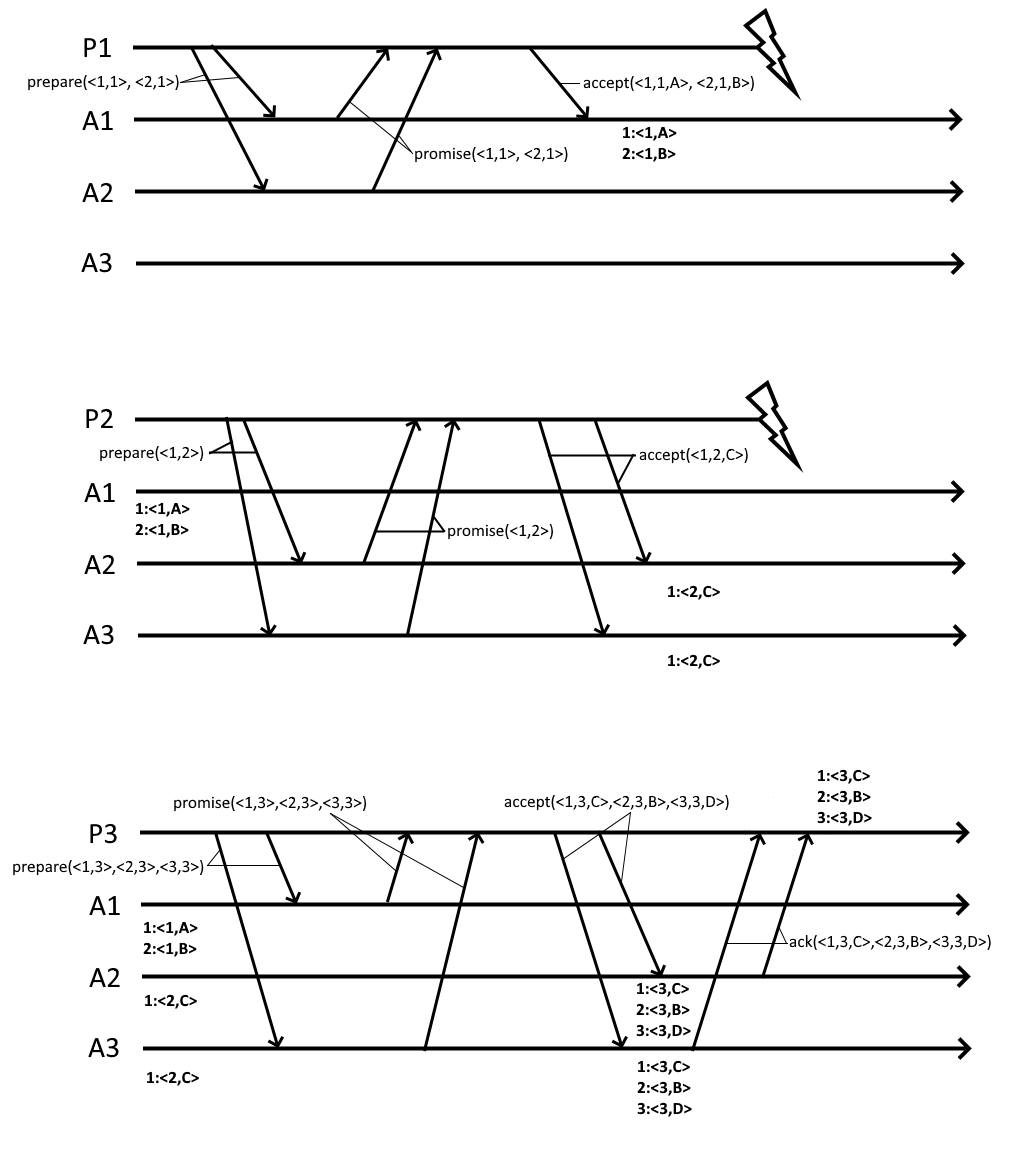
\includegraphics[width=\linewidth]{img/paxos_fail_2.png}
	\caption{Randfall von Paxos, bei dem sich die Reihenfolge von Zustandsänderungen ändern kann, nachdem sie bereits in einer anderen Reihenfolge von einen Proposer vorgeschlagen wurden. P1 schlägt die Werte A und B für die Indizes 1 und 2 vor. P3 schlägt jedoch die Werte C und B für die Indizes 1 und 2 vor und bekommt dafür eine Mehrheit. B könnte jedoch von A abhängig sein, da die Werte in dieser Reihenfolge von P1 vorgeschlagen wurden.}
	\label{fig:paxos_fail}
\end{figure}

\begin{figure}[H]
	\centering
	\includegraphics[width=\linewidth]{img/zab.png}
	\caption{Ablauf von Zab.}
	\label{fig:zab}
\end{figure}


Zab läuft im Gegensatz zu Paxos in drei Phasen ab (siehe \ref{fig:zab}):
\begin{enumerate}
	\item \textbf{Discovery}: Durch einen beliebigen Leader-Election-Algorithmus wird ein Kandidat für den Leader bestimmt. Alle anderen Server sind Follower. Alle Follower senden eine Nachricht mit der höchsten \textit{Epoch}-Nummer, die sie erhalten haben, an den Kandidaten. Wenn der Kandidat die \textit{Epoch}-Nummer von einer Mehrheit der Follower erhalten hat, schlägt er eine \textit{Epoch}-Nummer vor, die höher ist als alle, die er erhalten hat. Die Follower akzeptieren wiederum die vorgeschlagene \textit{Epoch}-Nummer und senden zusätzlich ihre History (das Log mit den bereits vorhandenen Transaktionen).
	Die Phase wird beendet, sobald die Merheit der Follower die \textit{Epoch}-Nummer akzeptiert haben und der Leader die History dieser Follower erhalten hat. Nun kann der Leader die aktuellste History bestimmen und diese in der nächsten Phase auf alle Follower replizieren. Durch die Discovery-Phase wird sichergestellt, dass die Follower keine kleinere \textit{Epoch}-Nummer akzeptieren.
	\item \textbf{Synchronization}: Der Kandidat schlägt sich selbst als Leader vor und sammelt Stimmen dafür ein. Dabei sendet der Leader auch die in der Discovery-Phase gewählte History, die auf die Follower repliziert wird. Wenn der Kandidat ein Quorum hat, wird er zum Leader und sendet eine \textit{Commit}-Nachricht an die Follower, die den Leader als gewählt anerkennen können und die Transaktionen in der vorher gesendeten History ausführen können. Durch diese Phase wird sichergestellt, dass sich die Server auf die History geeinigt haben und diese nicht mehr durch einen neuen Leader gelöscht werden kann.
	\item \textbf{Broadcast}: Der in der Synchronization-Phase etablierte Leader sendet neue Transaktionen an die Follower und sendet eine \textit{Commit}-Nachricht mit der Transaktion an alle Follower, sobald die Transaktion auf einer Mehrheit der Follower repliziert wurde. Sobald die Follower eine \textit{Commit}-Nachricht erhalten, können sie die entsprechende Transaktion ausführen. Diese Phase läuft ähnlich dem 2-Phase-Commit-Protokoll \cite{pc} ab. Die Verbindungen zwischen Leader und Followern wird über Heartbeats überwacht. Sobald ein Follower die Verbindung zum Leader verliert, startet er die Discovery-Phase. Wenn ein Leader die Verbindung zu einer Mehrheit der Server verliert, startet er ebenfalls die Discovery-Phase und gibt dadurch seine Leadership ab.
\end{enumerate}

\subsection{Raft}

Raft \cite{raft, raft-thesis} basiert ebenso wie Paxos auf dem Replicated-State-Machine-Modell basiert. Die Autoren begründen die Entwicklung von Raft damit, dass Paxos schwierig zu verstehen und zu implementieren sei. Deswegen wollten sie einen einfacheren Algorithmus entwickeln, der auf dem selben Modell basiert. Raft geht ebenso wie Paxos von einem Crash-Recovery-Modell und einem unzuverlässigen Netzwerk aus.
Im Gegensatz zu Paxos wird das Einigungsproblem bei Raft in drei Teilprobleme aufgeteilt:
\begin{itemize}
	\item \textbf{Leader Election}: Die Wahl eines Leaders ist bei Raft fester Bestandteil des Algorithmus 
	\item \textbf{Log Replication}: Das Log mit den Befehlen muss vom Leader auf die anderen Server des Cluster repliziert werden und es muss sich auf eine Reihenfolge geeinigt werden.
	\item \textbf{Safety}: Es muss Folgendes gelten: Alle Befehle müssen von allen Zustandsmaschinen in der gleichen Reihenfolge ausgeführt werden.
\end{itemize}

\subsubsection{Leader Election}

Ein Server hat immer einen der States \textit{Follower}, \textit{Candidate} oder \textit{Leader}. Alle Server starten als Follower. Raft teilt die Zeit in \textit{Terms} auf, die fortlaufend nummeriert werden. Jeder Term beginnt mit der Wahl eines Leaders. Jeder Server speichert seinen aktuellen Term und tauscht ihn bei jeder Kommunikation mit den anderen Servern aus. Wenn ein Server eine Anfrage mit einem alten Term bekommt, dann lehnt er diese ab. Wenn er eine Anfrage mit einem höheren Term bekommt, übernimmt er diesen und wird zum Follower. Eine Leader Election wird gestartet, wenn ein Follower eine Zeit lang keinen Heartbeat von einem Leader bekommt. Er wird dann zu einem Candidate und versucht Leader zu werden. Dabei startet er einen neuen Term, indem er seinen gespeicherten Term inkrementiert. Er sendet dann Vote Requests an alle anderen Server. Diese geben dem, Candidate ihre Stimme, falls sie ihre Stimme nicht bereits im selben Term einem anderen Server gegeben haben. Falls der Candidate von der Mehrheit der Server eine Stimme erhalten hat, wechselt er seinen Status zum Leader. So ist sichergestellt, dass es in einem Term maximal einen Leader geben kann. 

Es kann jedoch passieren, dass es in einem Term keinen Leader gibt. Falls mehrere Follower im gleichen Term eine Wahl starten (falls der Timer, der die letzte Nachricht von einem Leader überwacht, etwa zur gleichen Zeit ausläuft), kann es sein, dass es keine Mehrheit für einen Kandidaten gibt. Dann beginnen ein oder mehrere Candidates einen neuen Term und starten eine neue Wahl. Damit solche Konflikte selten vorkommen, sollten die Timeouts randomisiert werden, sodass es unwahrscheinlich ist, dass mehrere Server gleichzeitig eine Wahl starten.

Sobald ein Server sich zum Leader ernannt hat, kann er Anfragen von Clients bearbeiten und sendet periodisch Heartbeats an alle Follower, um seine Leadership aufrecht zu erhalten.

\subsubsection{Log Replication}

Im normalen Betrieb, d.h. ohne Leaderwechsel, nimmt der Leader Client-Anfragen an, schreibt diese ins Log und versucht sie, auf die Follower zu replizieren. Dazu sendet er sogenannte Append Entries Requests mit den Einträgen, die er replizieren möchte, an die Follower. Die Follower fügen diese in ihr eigenes Log ein und senden eine Bestätigung zurück, falls dies erfolgreich durchgeführt wurde. Der Leader merkt sich für jeden Follower einen \textit{Match Index}, der angibt, bis zu welchem Eintrag das Log des Followers dem des Leaders entspricht. Dadurch kann er feststellen, wann ein Eintrag auf eine Mehrheit der Server repliziert wurde. Sobald dies der Fall ist, kann er den Eintrag seiner State Machine übergeben und ausführen. Dann kann eine Antwort an den Client gesendet werden. Mit dem nächsten Append Entries Request oder Heartbeat wird der \textit{Commit Index} an die Follower weitergegeben, sodass diese den Eintrag ebenfalls ausführen können.

Nach einem Leader-Wechsel muss der Leader die Logs der Follower seinem eigenen Log angleichen. Dafür speichert er sich für jeden Follower einen \textit{Next Index}, der angibt, welcher Eintrag als nächstes an diesen Follower gesendet werden soll. Nach der Wahl zum Leader wird dieser für alle Follower auf den Index des letzten Eintrags initialisiert. Der Leader sendet außerdem bei jedem Append Entries Request den Term des letzten Eintrags, der vor den gesendeten Einträgen im Log ist, mit. Follower lehnen ein Append Entries Request ab, falls dieser Term nicht mit dem Term des Eintrags an diesem Index in ihrem Log übereinstimmt. Dann muss der Leader den \textit{Next Index} dieses Followers dekrementieren und es nochmal versuchen. Falls diese Überprüfung beim Follower nicht fehlschlägt und bereits inkonsistente Einträge vorhanden sind, werden alle folgenden Einträge gelöscht, sodass das Log dann bis zum Index des letzten gesendeten Eintrags dem des Leader entspricht.

\subsubsection{Safety}

Die zentrale Eigenschaft, die gelten muss damit das System korrekt funktioniert, ist: Sobald ein Log-Eintrag von einer State Machine ausgeführt wurde, darf keine andere State Machine auf einem anderen Server einen anderen Befehl für diesen Log-Eintrag ausführen. Dadurch wird offensichtlich sichergestellt, dass alle State Machines die Befehle in der gleichen Reihenfolge bearbeiten. Diese Eigenschaft ist in Raft äquivalent zu: Wenn ein Leader entscheidet, dass ein Eintrag \textit{committed} ist und diesen der State Machine übergibt, dann muss dieser Eintrag in den Logs aller zukünftigen Leadern vorhanden sein. Dies wird durch zusätzliche Einschränkungen beim Committen und bei der Leader Election erreicht.

\begin{itemize}
	\item \textbf{Leader Election}: Die Candidates senden mit ihren Vote-Requests den Term und Index des letzten Eintrags ihres Logs mit, anhand derer die wählenden Server entscheiden, ob sie dem Candidate ihre Stimme geben oder nicht. Damit Log Einträge, die auf einer Mehrheit der Server repliziert sind, nicht gelöscht werden, gibt der Server dem Candidate keine Stimme, falls sein Log kompletter ist, d.h. falls der Term des letzten Eintrags größer ist oder falls der Term gleich ist und der Index größer ist. Dadurch hat der nächste Leader dann das kompletteste Log unter einer Mehrheit der Server.
	\item \textbf{Commit}: Um einen Eintrag zu committen, muss mindestens ein Eintrag aus dem aktuellen Term des Leaders auf einer Mehrheit der Server repliziert worden sein. Sonst kann es passieren, dass ein Server Leader wird, der die auf einer Mehrheit replizierten Einträge nicht in seinem Log hat, da er nur neuere Einträge in seinem Log hat. Abbildung \ref{fig:zab} zeigt einen solchen Fall: Die Einträge in Index 2 und 3 mit Term 2 sind auf einer Mehrheit der Server repliziert. Falls Server 2 jedoch Leader in Term 4 wird, darf er diese Einträge nicht committen. In Term 5 kann Server 1 Leader werden, da er das längste Log hat. Er würde dann die Logs der Follower seinem anpassen und die Einträge mit Term 2 würden gelöscht werden. Sobald Server 2 jedoch einen Eintrag in seinem aktuellen Term (Term 4), auf Server 3 repliziert hat, kann Server 1 nicht mehr in Term 5 Leader werden. Jetzt können die Einträge in den Indizes 2-4 committet werden.
\end{itemize}

\begin{figure}[H]
	\centering
	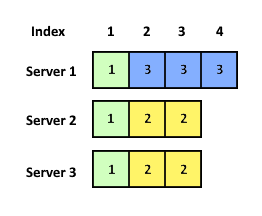
\includegraphics{img/raft-log.png}
	\caption{Log-Einträge von drei Raft-Servern. Die Zahl in den Einträgen gibt den Term des Eintrags an.}
	\label{fig:zab}
\end{figure}
\chapter{Implementierung}
\label{impl}

\section{Überblick}

Um ein System wie in \ref{ziele} beschrieben zu entwickeln, muss zunächst ein Algorithmus festgelegt werden, der die gewünschten Eigenschaften hat. Dieser Algorithmus wird den Kern des Systems bilden. In \ref{algo} wird diese Entscheidung erläutert. Dann wird in \ref{sprache} die Wahl der Programmiersprache erklärt und in \ref{konzept} auf die grundlegenden Konzepte des zu entwickelnden Systems eingegangen.

\subsection{Wahl des Algorithmus}
\label{algo}

Die Kandidaten sind die in \ref{algos} vorgestellten Algorithmen Paxos, Zab und Raft. Die Beschreibung von Paxos ist sehr theoretisch und nicht praxisnah gehalten, was zu Problemen bei der Implementierung führen könnte, die nicht im Dokument beschrieben sind und für die somit zeitaufwändig eigene Lösungen entworfen werden müssten. Dies bestätigen die wenigen Paxos-Implementierungen und die Berichte von Autoren, die auf Paxos basierende Systeme entwickelt habe und von Schwierigkeiten bei der Implementierung berichten. Zab wurde speziell für Zookeeper entwickelt und wurde soweit bekannt in keinem anderen System implementiert. Der Vorteil von Zab gegenüber Paxos und Raft, dass nebenläufige Anfragen von Clients die Reihenfolge nicht ändern können, ist zumindest für einfache Koordinierungsaufgaben, wie sie das System für DXRAM übernehmen soll, nicht relevant. Falls diese Eigenschaft im Nachhinein benötigt werden sollte, könnte man dies, wie die Autoren von Zab auch anmerken, mit Paxos oder Raft ebenfalls implementieren. Die Beschreibung von Raft ist sehr praxisnah und es wird auf viele Implementierungsdetails eingegangen. Außerdem sind bereits einige Implementierungen vorhanden, was darauf schließen lässt, dass Raft einfacher zu implementieren ist als Paxos. Deshalb wurde Raft als Algorithmus für das zu entwickelnde System ausgewählt.

\subsection{Wahl der Programmiersprache}
 \label{sprache}

Als Programmiersprache für das zu entwickelnde System wurde Java gewählt. Java ist eine in der Industrie weit verbreitete Sprache, die für die es viele gut entwickelte Tools und Bibliotheken gibt. Ein Vorteil gegenüber dynamischen Programmiersprachen wie Python ist auch die Typsicherheit, die bereits zur Compilezeit sichergestellt wird. Dies kann bei der Erkennung von subtilen Fehlern im Code helfen, was bei eher komplexeren Systemen wie einem Einigungsalgorithmus wichtig ist. Außerdem erleichtert die Wahl von Java die vorgesehene Integration in DXRAM, da DXRAM ebenfalls in Java implementiert ist. Für das Build-Management wird Gradle verwendet.

\subsection{Konzept der Implementierung}
 \label{konzept}
 
Die Implementierung soll möglichst performant sein und später Möglichkeiten zur Optimierung bieten. Dazu ist es sinnvoll, sie möglichst leichtgewichtig zu gestalten und keine großen Frameworks oder Bibliotheken zu verwenden. Außerdem soll die Nutzung möglichst einfach sein. Insbesondere sollte das Bootstrapping möglichst automatisch ablaufen können, sodass der Einsatz in einem verteilten System keine zusätzlichen Tools benötigt.

Das System besteht aus Server-Instanzen und Clients. Die Server-Instanzen bilden ein Cluster und führen den Einigungsalgorithmus aus. Die Clients verbinden sich mit dem Cluster und bieten dem Nutzer eine Schnittstelle zum System an. Server und Clients sollen sowohl Standalone als auch als Bibliothek genutzt werden können. Das nutzen als Bibliothek hat den Vorteil, dass für das System kein eigener Prozess gestartet werden muss.

Die Schnittstelle soll auf unterster Ebene eine Speicherung von Key-Value-Daten ermöglichen. Die Daten sollen mit einem String identifiziert werden und Daten von beliebigem Typ speichern. Außerdem sollen beliebige atomare Operationen auf den Daten ausgeführt werden können. Mit dieser Schnittstelle könnten dann weiter abstrahierte Funktionalitäten bzw. Klassen implementiert werden, wie z.B. eine \textit{DistributedAtomicInteger}-Klasse, die atomare Operationen auf einem im System gespeichertem Integer-Wert ausführt.

Da das System in DXRAM verwendet werden soll, speziell dafür entwickelt wird und Raft als Einigungsalgorithmus nutzen wird, soll das System DXRaft heißen.

\section{Server}

Die Server-Instanzen bilden das Raft-Cluster und führen den Raft-Algorithmus durch. Dafür müssen sie die im Raft-Algorithmus definierten Daten speichern und zwischen den Status wechseln können. Ein Server kann mit der \textit{RaftServer}-Klasse erstellt und gestartet werden. Im Folgenden werden die Probleme erläutert, die bei der Implementierung aufgekommen sind, und die Konzepte erklärt, mit denen diese gelöst wurden.

\subsection{Messaging}
\label{messaging}

Da DXRaft ein verteiltes System ist, müssen die Instanzen über das Netzwerk kommunizieren. Um diese zu implementieren gibt es offensichtlich viele verschiedene Ansätze. Um bessere Möglichkeiten zur Optimierung zu bieten und die Implementierung leichtgewichtig zu halten, wird hier auf die Verwendung von fertigen Implementierungen wie DXNet oder MPI verzichtet.

Zunächst muss ein Transportschichtprotokoll festgelegt werden, mit dem die Kommunikation ablaufen soll. 
Der Raft-Algorithmus nutzt eine Nachrichtensemantik, das heißt die Server senden sich gegenseitig einzelne Nachrichten und keinen Strom von Daten. Außerdem wurde beim Entwurf des Algorithmus bereits ein unzuverlässiges Netzwerk berücksichtigt und erlaubt verlorene Nachrichten. Deshalb wird in DXRaft UDP genutzt. Das Messaging ist jedoch mithilfe von \textit{NetworkService}-Interfaces modular aufgebaut, sodass der Nachrichtenaustausch nachträglich auch anders implementiert werden könnte. Es könnte z.B. sinnvoll sein, TCP-Verbindung zwischen den Raft-Servern aufzubauen, um die Verbindungen zu überwachen und schnell Ausfälle zu erkennen. Da in einem Raft-Cluster normalerweise eine eher kleine Anzahl an Servern teilnimmt, ist der Aufwand für das Verwalten der Verbindungen zu vernachlässigen. Bei der Verbindung von den Clients zum Server könnten das Verwalten der Verbindungen jedoch zu einem Problem werden: Alle Anfragen müssen stets über den Leader geleitet werden. In DXRaft sendet jeder Client seine Anfragen direkt an den Leader. Wenn TCP verwendet werden würde, müssten alle Clients eine Verbindung zum Leader aufbauen. Man könnte die Last jedoch vom Leader nehmen, indem auch die Follower Client-Verbindung halten können und dann das Weiterleiten an den Leader übernehmen. 

Da an die interne Kommunikation andere Anforderungen gestellt sind als an die externe Kommunikation mit Clients, sind diese in DXRaft getrennt und es wird jeweils ein eigener Socket geöffnet. Jeder Socket wird von jeweils einem Thread überwacht, der die Nachrichten deserialisiert und je nach Nachrichtentyp verarbeitet. Um die Performance des gesamten Systems zu verbessern, wäre es eventuell sinnvoll, mehrere Threads pro Socket einzusetzen, um Nachrichten parallel zu verarbeiten.

Da UDP zum Senden von Anfragen genutzt wird, muss das erneute Senden auf der Anwendungsebene übernommen werden. Dafür überwacht der Leader für jeden \textit{Append Entries}- und \textit{Vote-}Request an die Follower die Zeit bis zur Antwort. Falls er die Antwort nicht rechtzeitig erhält, sendet er die Anfrage erneut. Die Anfragen und Antworten werden mit einer aufsteigenden Zahl identifiziert, die der Leader beim Senden vergibt. Um die Korrektheit zu garantieren, sendet der Leader momentan an jeden Follower höchstens eine Anfrage gleichzeitig. Mit einem \textit{Append Entries}-Request können jedoch mehrere Log-Einträge versendet werden, falls während eines Anfrage-Antwort-Zyklus bereits mehrere Einträge an das Log angehangen wurden. Auch hier könnte man die Perfomance möglicherweise erhöhen, indem mehrere parallele Anfragen an die Follower erlaubt werden. Dann müsste jedoch sichergestellt werden, dass die Anfragen vom Follower in der richtigen Reihenfolge verarbeitet werden (z.B. durch Verwendung von TCP) und eine Flusskontrolle implementiert werden, die die Anzahl der parallel gesendeten Anfrage vorgibt.

\subsection{Bootstrapping}

Um den Raft-Algorithmus durchzuführen und insbesondere festzustellen, wann eine Mehrheit der Server eine Anfrage akzeptiert hat, muss jeder teilnehmender Server alle anderen teilnehmenden Server kennen. Diese Information muss den Servern beim Bootstrapping bekannt gemacht werden. Eine einfache Möglichkeit ist, jeder Server-Instanz alle teilnehmenden Server mit ihren Adressen \textbf{statisch} beim Start per Konfigurationsdatei zu übergeben. Dies wird so auch in einigen Systemen, wie z.B. Zookeeper, so gelöst und ist auch in DXRaft eine Möglichkeit, die Server zu starten. 

Dies ist jedoch nicht sehr komfortabel, da alle teilnehmenden Server mit ihren Adressen manuell oder mit einem eigens dafür geschriebenem Skript eingetragen werden müssen. Deshalb gibt es in DXRaft die Möglichkeit, dass die Server sich automatisch finden und den Cluster \textbf{dynamisch} aufbauen. Dazu muss eine Server-Instanz als Bootstrap-Instanz gewählt, die damit beginnt, ein Cluster aufzubauen. Er fügt sich selbst in die Liste der teilnehmenden Server ein und erstellt dafür einen Log-Eintrag, der über den normalen Raft-Mechanismus später auf alle teilnehmenden Server repliziert wird. Dann öffnet er einen Multicast-Socket und wartet, bis er darüber \textit{Join-Requests} von anderen Server erhält. Ein \textit{Join-Request} beinhaltet die Adresse des Servers, der dem Cluster beitreten möchte, sodass das Beitreten über den Beitrittsmechanismus (beschrieben in \ref{config-change}) gestartet werden kann. Da jeder beitretende Server dadurch auch das gesamte Log übergeben bekommt, bekommt er auch die Adressen aller Server mitgeteilt, die bereits vor ihm dem Cluster beigetreten sind. Falls die Bootstrap-Instanz, die initial der Leader ist, abstürzt, nachdem bereits ein oder mehrere Server dem Cluster beigetreten sind, wird der nächste Leader zur Bootstrap-Instanz. So kann der Boot-Vorgang auch weiterhin fortgeführt werden.

Außerdem müssen die Server eindeutig identifiziert werden, damit der Raft-Algorithmus korrekt funktioniert. Deshalb hat jede Server-Instanz in DXRaft einen Integer-Identifier \textit{id}. Bei statischer Konfiguration muss die \textit{id} in der Konfigurationsdatei mit den Adressen der Server übergeben werden. Bei dynamischer Konfiguration werden die \textit{ids} ebenfalls dynamisch vergeben. Dazu wird wieder der Raft-Mechanismus selber verwendet: Die Bootstrap-Instanz gibt sich selbst die \textit{id} 0 und erstellt einen \textit{Atomic Integer}-Eintrag für die Vergabe der \textit{ids}. Die Server, die dem Cluster beitreten wollen, müssen sich dann zunächst nach dem Start eine \textit{id} besorgen. Dafür senden sie über IP-Multicast einen \textit{Assign-Id-Request}. Wenn die Bootstrap-Instanz (oder der aktuelle Leader) die Anfrage bekommt, führt ein atomares \textit{GetAndIncrement} auf dem \textit{Atomic Integer}-Eintrag durch und sendet die erhaltene \textit{id} zurück. Dann kann der Server den Beitritt zum Cluster wie bereits beschrieben starten.

Wie bei Client-Anfragen muss auch bei \textit{Join-Requests} und \textit{Assign-Id-Request} über Multicast sichergestellt werden, dass diese nicht doppelt durchgeführt werden, falls der Sender keine Antwort auf seine Anfrage bekommt und die selbe Anfrage erneut sendet. Dazu bekommt jede Anfrage eine UUID \cite{uuid}. Eine dedizierte Session wird bei der Bootstrap-Instanz verwendet, um die Multicast-Anfrage und die Ergebnisse zu speichern, sodass diese nicht doppelt ausgeführt werden können (siehe \ref{sessions} für die Erklärung des Session-Mechanismus bei (Client-)Anfragen)). Diese dedizierte Session ist momentan unbegrenzt groß, da es normalerweise nicht allzu viele Multicast-Anfragen geben sollte, sodass sie den Speicher nicht zu sehr belastet. Die UUID wird auch mit der Antwort gesendet, damit der anfragende Server die Antwort identifizieren kann.

Die statische Konfiguration ist etwas sicherer, falls einer oder mehrere  Server bereits während des Boot-Vorgangs abstürzen sollten. Da alle Server bereits alle Server kennen, können keine Anfragen bearbeitet werden, wenn keine Mehrheit erreicht werden kann. Bei dynamischer Konfiguration ist bei Anfragen während des Boot-Vorgangs nicht sichergestellt, dass bereits alle Server dem Cluster beigetreten sind. Falls dies nicht der Fall ist, dann ist die Fehlertoleranz eventuell schlechter als erwartet, da weniger Server am Cluster teilnehmen und die Mehrheit anders berechnet wird. Dies könnte gelöst werden, indem dem Cluster eine Zahl übergeben wird, die angibt, ab welcher Anzahl an beigetretenen Servern Anfragen beantwortet werden können. Dann kann jedoch ein einziger Server, der ausfällt, den Boot-Vorgang fehlschlagen lassen.

Aus diesen Gründen kann man je nach Anforderungen per Parameter das Bootstrapping statisch oder dynamisch durchführen.

\subsection{Persistenz}

Im Raft-Algorithmus ist es vorgesehen, dass sich Server nach einem Absturz wieder erholen können und nach einem \textit{Recover}-Vorgang wieder am Cluster teilnehmen können, ohne das korrekte Arbeiten des Algorithmus zu stören. Dazu müssen wichtige Daten, wie z.B. der \textit{current term} oder das Log, synchron auf Festplatte gesichert werden, sodass diese bei einem möglichen Absturz nicht verloren gehen. Dies ist in DXRaft noch nicht implementiert und das Wiederherstellung wird moment dem Systemadminstrator überlassen (z.B. durch das Entfernen und erneute Hinzufügen des Servers zum Cluster über den Beitrittsmechanismus).

Dennoch muss das Log bereits ohne die Möglichkeit der Wiederherstellung persistiert werden: Da bei jeder Anfrage ein Eintrag in das Log geschrieben wird, wird das Log schnell sehr groß. Falls das Log nur im Speicher gehalten wird, belastet es auch sehr stark den Garbage Collector und die Garbage-Collector-Pausen werden sehr lang (\textgreater 500 ms), wodurch die Timeouts nicht mehr richtig funktionieren und es zu unnötigen Leaderwechseln kommt. Außerdem kann das Log dann auch schnell den gesamten Speicher ausfüllen. Deswegen ist es nötig, das Log auf Festplatte zu persistieren.

Da Festplattenzugriffe sehr viel mehr Zeit benötigen als Speicherzugriffe, muss das Log möglich effizient gespeichert werden und die Zugriffe minimiert werden, damit die Performance nicht zu sehr leidet.

Das Log muss durch das Replizieren auf die anderen Server gelesen werden können. Insbesondere wird auf die neuesten Einträge häufig zugegriffen, während es unwahrscheinlich ist, dass auf ältere Einträge zugegriffen werden muss. Dennoch muss das Log theoretisch bis zum Anfang gelesen werden können, da Follower beliebig viele Nachrichten des Leaders nicht bekommen und dadurch beliebig viele Einträge nicht mitbekommen könnten. Um diese dann auf die betroffenen Follower zu replizieren, sobald diese wieder Nachrichten erhalten, müssen alte Einträge gelesen werden. Außerdem muss bei einem Beitritt eines neuen Servers das gesamte Log auf den neuen Server übertragen werden.

Weiterhin müssen auch Einträge am Ende des Logs gelöscht werden können. Dies kann bei Leaderwechseln nötig werden, wenn der Leader die Logs der Follower seinem Log angleicht und es Einträge gibt, die im Log des Followers vorhanden sind aber nicht im Log des Leaders.

Die Einträge des Logs sind beliebig groß, weswegen die Länge der Einträge in der Log-Datei mitgespeichert werden muss, um die Einträge wiederzufinden. Dadurch kann nicht direkt mit einem Index auf den entsprechenden Eintrag zugegriffen werden. Die naive Lösung ist, die Länge des Eintrags immer vor dem Eintrag zu speichern und beim Lesen eines Eintrags die Log-Datei von Beginn an zu durchsuchen, indem immer die Länge des nächsten Eintrags gelesen wird und diese Anzahl an Bytes übersprungen wird, bis der gesuchte Eintrag gefunden wurde. Dies ist aber offensichtlich keine gute Lösung, das Suchen eines Eintrags dadurch linear mit der Länge des Logs steigt.

Eine weitere Möglichkeit wäre es, eine zusätzliche Datei anzulegen, die zu jedem Index die Adresse des Eintrags in der Log-Datei speichert. Dann könnte der Zugriff in konstanter Zeit erfolgen, falls man davon ausgeht, dass die Indexdatei in konstanter Zeit gelesen werden kann. Dann müsste jedoch beim Anhängen eines Log-Eintrags mindestens zwei Mal auf die Festplatte geschrieben werden, einmal um den Eintrag in die Log Datei zu schreiben und einmal um die Adresse in die Indexdatei zu schreiben. Da die Zugriffe wegen der Fehlertoleranz immer synchron geschehen müssen, erhöhen sie die Latenz von Client-Anfragen deutlich. Deshalb wäre es gut, wenn das Anhängen auf einen Schreib-Zugriff reduziert werden könnte.

Dafür nutzt DXRaft die bereits vorhandene Baumstruktur des Dateisystems. Das Log wird in mehrere Dateien aufgeteilt, die eine maximale Größe haben. Sobald das Anhängen eines Log-Eintrags die maximale Größe der Log-Datei überschreiten würde, wird eine neue Log-Datei angelegt und der Eintrag in diese neue Datei geschrieben. Der Index des ersten Eintrags, der in der dieser Datei gespeichert ist, wird im Namen der Datei gespeichert. Beim Lesen eines Eintrags kann dann mithilfe des Verzeichnisses die Datei ermittelt werden, in der dieser Eintrag gespeichert ist. Die Datei kann dann wie in der naiven Lösung nach dem Eintrag durchsucht werden. Dadurch ist das Lesen durch die maximale Größe einer Log-Datei beschränkt und das Schreiben benötigt normalerweise nur einen Schreibzugriff. Dazu kommt nur das Anlegen einer neuen Datei, falls eine Log-Datei zu groß geworden ist. Um die Schreib- und Lesezugriffe auf die Festplatte weiter zu minimieren, wird außerdem gepuffert gelesen und geschrieben (mit den \textit{BufferedReader}- und \textit{BufferedWriter}-Klassen aus dem \textit{java.io}-Package).
		
Dies könnte durch Batch-Verarbeitung von Anfragen noch weiter reduziert werden, wobei dann nur ein Schreibzugriff für das Anhängen mehrerer Einträge nötig wäre. Da dies jedoch nicht ganz einfach zu implentieren ist und die Performance auch ohne Batch-Verarbeitung bereits ausreichend ist, wurde dies im Rahmen dieser Arbeit noch nicht implementiert.

Da die neuesten Einträge des Logs häufig gelesen werden müssen, werden diese außerdem noch in einem Cache gehalten. Der Cache hält die letzten \textit{n} Einträge im Speicher und es wird der älteste entfernt, falls der Cache voll ist und ein neuer Einträg an das Log angehängt wird. Da im Normalbetrieb nur auf die neuesten Einträge zugegriffen wird, kann durch einen ausreichen großen Cache erreicht werden, dass im Normalbetrieb kein Lesezugriff auf die Festplatte erfolgt.

Da auch auf der Festplatte nicht unendlich Speicherplatz vorhanden ist, kann das Log auch diesen Platz irgendwann aufbrauchen. Damit das System dann weiterhin funktioniert, muss eine Kompaktierung des Logs implementiert werden. Dazu haben die Raft-Autoren ebenfalls einen Mechanismus entwickelt, der jedoch in DXRaft noch nicht implementiert wurde.

\subsection{Änderungen der Clusterkonfiguration}
\label{config-change}

Im laufenden Betrieb kann es vorkommen, dass man die Menge der am DXRaft-Cluster teilnehmenden Server ändern möchte, z.B. möchte man einen ausgefallenen Server durch einen neuen ersetzen. Währenddessen sollte das Cluster nach Möglichkeit weiterhin funktionieren und Anfragen beantworten. Wenn in einer Konfigurationsänderung mehrere Server dem Cluster beitreten oder aus dem Cluster austreten, kann es passieren, dass während der Konfigurationsänderung zwei Mehrheiten für entstehen, da die Konfigurationsänderung nicht allen Servern im Cluster gleichzeitig bekannt gemacht werden kann. Daraus könnte dann resultieren, dass zwei Leader in einem Term existieren. Das würde die Sicherheitsbedingung von Raft verletzten und zu Inkonsistenzen führen.

Die von den Raft-Entwicklern vorgeschlagene Lösung ist, nur einem Server gleichzeitig zu erlauben, dem Cluster beizutreten oder aus dem Cluster auszutreten. Dabei können keine zwei Mehrheiten gleichzeitig entstehen. Wenn mehrere Server dem Cluster beitreten wollen, müssen das Beitreten sequentiell ablaufen. Diesen Mechanismus nutzt auch DXRaft.

Ein Beitritt eines Servers kann entweder von dem Server selbst oder von einem Client initiiert werden. Wenn der Server selbst den Beitritt initiiert, sendet er einen \textit{JoinServer}-Request über IP-Multicast. Falls Broadcast in der Konfigurationsdatei deaktiviert ist, startet der Server im Idle-Modus wartet auf Nachrichten des Leaders. Dann muss ein Client den Beitritt initiieren, indem er einen \textit{AddServer}-Request mit der Adresse beitretenden Servers sendet. Unabhängig davon, wer den Beitritt initiiert, läuft der Beitritt gleich ab: Der Leader prüft zunächst, ob bereits eine Konfigurationsänderung läuft. Falls dies der Fall ist, wird die Anfrage in eine Warteschlange eingefügt. Sobald die laufende Konfigurationsänderung abgeschlossen ist, wird die nächste Änderung gestartet. Auch für Konfigurationsänderungs-Anfragen wird das Log genutzt, um diese allen Servern konsistent bekannt zu machen. Es wird ein Log-Eintrag für jede Konfigurationsänderung angelegt und sobald diese der Eintrag auf einer Mehrheit der Server repliziert wurde, ist die Änderung abgeschlossen und kann beantwortet werden. Die Server fügen den beitretenden Server in ihre Liste der bekannten Server ein, sobald sie den entsprechenden Eintrag an ihr Log anhängen. Der neue Server bekommt über den normalen Replikations-Mechanismus mit \textit{AppendEntries}-Requests das gesamte Log geschickt, sobald er dem Leader bekannt ist.

Ein Austreten eines Servers muss von einem Client initiiert werden. Der Austritt läuft analog zum Beitritt ab. Sobald der Austritt vom Leader bestätigt wurde, kann der Server abgeschaltet werden. Ein automatisches Ausschließen von nicht antwortenden Servern aus dem Cluster ist problematisch, da nicht festgestellt werden kann, ob der Server abgestürzt ist oder nur die Nachrichten verloren gehen. Dadurch könnte es passieren, dass ein Server ausgeschlossen wird, obwohl er noch aktiv ist. Dieser könnte dann die Arbeit des restlichen Clusters beeinträchtigen, z.B. indem er periodisch eine Leader-Wahl initiiert. Außerdem würde durch ein automatisches Verkleinern des Clusters der Replikationsgrad verringert werden, wodurch das System an Sicherheit verliert.

Zur Optimierung des Beitritts könnte noch ein zusätzlicher \glqq Recovery \grqq-Mechanismus implementiert werden, durch den das Log des neuen Servers auf den Stand des Logs des Leaders gebracht wird bevor der Beitritt gestartet wird. Da dabei das gesamte Log an den neuen Server geschickt werden muss, wäre es sinnvoll das Lesen und Senden vieler Log-Einträge optimiert werden, z.B. durch paralleles Lesen aus der Log-Datei. Diese Optimierungen wären bei dem normalen Replikations-Mechanismus nicht sinvoll, da dabei die Server meist nicht so viele Einträge erhalten müssen und die Einträge auch meistens aus dem Cache gelesen werden können.

\subsection{Timer}

Die Server müssen aus unterschiedlichen Gründen die Zeit im Auge behalten und einen Timeout auslösen, falls ein Ereignis zu lange auf sich warten lässt:

\begin{itemize}
	\item Leader müssen periodisch einen Heartbeat senden, falls das System gerade keine Anfragen bearbeitet und das System gerade keine Anfragen bearbeitet.
	\item Candidates müssen eine neue Wahl starten, wenn die Wahl in einer Zeitspanne keinen Sieger hervorgebracht hat.
	\item Follower müssen einen eine Wahl starten, wenn sie zu lange keine Nachricht vom Leader erhalten haben.
\end{itemize}

Diese Funktionalität wird durch die \textit{RaftTimer}-Klasse bereitgestellt. Diese verwendet intern einen \textit{ScheduledExecutorService}, der, wenn aktiviert, auslöst, sobald eine vorher übergebene Zeit abgelaufen ist. Dann wird die \textit{processTimeout()}-Methode eines vorher übergebenen \textit{TimeoutHandlers} aufgerufen. 

Damit die Server im Cluster möglichst nicht zur gleichen Zeit einen Timeout auslösen, sollte die Zeitspanne randomisiert werden. Dafür kann der \textit{RaftTimer}-Klasse ein fixe Zeit \textit{f} und zusätzliche randomisierte Zeit \textit{r} übergeben werden. Der Timer löst dann frühestens aus, nachdem \textit{f} abgelaufen ist, und spätestens, nachdem \textit{f+r} abgelaufen ist.

Außerdem wird der Timer auch für die Überwachung von \textit{Append Entries}- und \textit{Vote-}Requests genutzt. Diese müssen nach dem Ablauf des Timers erneut gesendet werden, falls der Leader in dieser Zeit keine Antwort erhalten hat (siehe \ref{messaging}).

\section{Client}

Der Client bildet die Schnittstelle von DXRaft zur Anwendung. Er wird als Library in die Anwendung eingebunden und leitete die Anfragen von der Anwendung an das DXRaft-Cluster weiter. Standardmäßig werden die DXRaft-Server automatisch über Multicast gefunden. Falls dies nicht möglich, muss dem Client eine Liste der Server mit Adressen übergeben werden. Bei der Implementierung des Clients ist es vor allem wichtig, dass Fehler, wie z.B. das Ausbleiben einer Antwort von einem Server, korrekt behandelt wird. In \ref{sessions} wird beschrieben, wie es erreicht werden kann, dass die Anfragen immer genau ein mal ausgeführt werden. In \ref{api} wird dann die API genau beschrieben.

\subsection{Sessions}
\label{sessions}

Wenn der Client keine Antwort auf seine Anfrage bekommt, dann kann er nicht feststellen, ob die Anfrage erfolgreich durchgeführt wurde oder nicht. Wenn er dann sofort aufgeben würde, wäre das System nicht fehlertolerant. Deswegen sendet er die gleiche Anfrage erneut, um dem Server zu signalisieren, dass er keine Antwort erhalten hat. Dies könnte jedoch ohne weitere Maßnahmen dazu führen, dass die Anfrage mehrfach bearbeitet wird. Das wäre für den Nutzer jedoch unerwartet und würde bedeuten, dass das System nicht korrekt arbeitet. Um die mehrfache Bearbeitung einer Anfrage zu verhindern, müssen die Anfragen mit dem Ergebnis serverseitig gespeichert werden, sodass der Server feststellen kann, ob er die Anfrage bereits einmal erhalten hat und das Ergebnis zurücksenden kann, falls diese bereits durchgeführt wurde.

Leider können nicht alle Anfragen mit dem Ergebnis gespeichert werden, da dann das gesamte Log im Speicher gehalten werden müsste und auch bei jeder Anfrage komplett durchsucht werden müsste. Um diese Problematik zu lösen, werden die Daten in Sessions gespeichert, die eine begrenzte Anzahl Anfragen mit dem Ergebnis speichern. Jeder Client sendet dafür einen \textit{CreateSession}-Request an das Cluster, bevor er irgendeine andere Anfrage stellt. Er bekommt dann die Session-Id der erstellten Session zurück. Jede Anfragen bekommt dann vom Client die Session-Id, die die Session der Anfrage identifiziert, und eine aufsteigenen Integer-Id, die die Anfrage in der Session identifiziert, zugewiesen. Dadurch ist jede Anfrage eindeutig identifiziert und kann wiedergefunden werden.

Wenn der Client so viele Anfragen gesendet hat, dass seine Session voll ist, werden seine Anfragen nicht mehr bearbeitet und der Server sendet einen \textit{SESSION\textunderscore FULL}-Error zurück. Dann muss die Session geleert werden. Dazu muss der Client zunächst sichergehen, dass er zu allen ausstehenden Anfragen eine Antwort erhalten hat. Dann kann er einen \textit{PurgeSession}-Request senden, mit dem die Session geleert wird. Sobald dies erfolgreich geschehen ist, kann er weitere Anfragen stellen.

Da nicht unendlich viele Sessions im Speicher gehalten werden, müssens Sessions irgendwann auslaufen. Dies geschieht in DXRaft sobald eine bestimmte Zahl an Sessions erreicht ist. Dann wird die älteste Session invalidiert. Falls der Client der Session noch aktiv ist und eine weitere Anfrage sendet, wird ein \textit{SESSION\textunderscore EXPIRED}-Error gesendet. Es könnte dann Folgendes passiert sein: Die Anfrage wurde ausgeführt, die Antwort ist jedoch verloren gegangen. Bevor der Client die Anfrage erneut sendet, erstellt ein anderer Client eine Session. Da der Session-Speicher voll ist, muss die Session des ersten Clients gelöscht werden. Als dieser Client die vorherige Anfrage erneut sendet, bekommt er einen \textit{SESSION\textunderscore EXPIRED}-Error zurück. Die Anfrage wurde jedoch ausgeführt. Der Client kann dann also nicht mehr feststellen, ob seine Anfrage ausgeführt worden ist oder nicht. Deshalb wirft der Client in diesem Fall eine \textit{SessionExpiredException}. Es wird also dem Nutzer überlassen, wie dieser Fall behandelt werden soll. 

Durch die Anpassung der maximalen Anzahl an Sessions an die Anforderungen sollten sich ausgelaufene Sessions von aktiven Clients vermeiden lassen. Es könnten auch andere Verdrängungsstrategien für den Session-Speicher implementieren wie z.B. Least-Recently-Used or zeitbasierte Invalidierung. Bei zeitbasierter Invalidierung müsste jedoch sichergestellt werden, dass sich das gesamte DXRaft-Cluster auf die Zeit einigt, ab der die entsprechende Session invalidiert wird.

Damit die Sessions dem gesamten DXRaft-Cluster bekannt sind und bei einem Leaderwechsel weiter funktionieren, werden die \textit{CreateSession}- und \textit{PurgeSession}-Requests genau so behandelt wie andere Anfragen, das heißt sie werden mit dem Raft-Mechanismus repliziert und erst ausgeführt, wenn sie auf eine Mehrheit der Server repliziert wurden. Dadurch werden die Sessions auf jedem Server erstellt und die Server sind sich einig, wann eine Session geleert oder gelöscht wird.


\subsection{API}
\label{api}

Die \textit{RaftClient}-Klasse bildet die Schnittstelle zu DXRaft. Es werden Methoden zum Lesen, Schreiben und Löschen von Daten angeboten. Die Daten werden mit einem String identifiziert. Das Datenobjekt, das in DXRaft gespeichert werden soll, muss das \textit{RaftData}-Interface implementieren. Implementierungen für die meisten Standarddatentypen sind im Package \textit{de.hhu.bsinfo.dxraft.data} zu finden. 

Beim Lesen kann über einen Boolean-Wert bestimmt werden ob das Lesen von alten Daten erlaubt ist. Falls dies der Fall ist, wird die Anfrage nicht an den Leader sondern an einen beliebigen DXRaft-Server geschickt. Dieser liest die Daten direkt aus seinen aktuellen Status aus und hängt die Leseanfrage nicht an das Raft-Log an. Dadurch kann die Anfrage schneller bearbeitet und Last vom Leader genommen werden. Die gelesenen Daten können jedoch beliebig alt sein, da nicht klar ist, wie weit der antwortende Server dem Leader hinterherhängt. Falls das Lesen von alten Daten nicht erlaubt wird, durchläuft die Leseanfrage den normalen Raft-Mechanismus, das heißt die Anfrage wird an den Leader gesendet, an das Log angehängt und repliziert. Dadurch ist die Konsistenz des Lesens garantiert.

Da bei allen Anfragen Fehler auftreten können, müssen diese dem Nutzer mitgeteilt werden. Dafür geben alle Methoden eine Wrapper-Objekt zurück, welches das Ergebnis der Anfrage und einen möglichen Error-Code enthält. So kann nach einer Anfrage jeweils überprüft werden, ob es einen Fehler bei der Bearbeitung gab. Dann kann enstprechend dem Error-Code gehandelt werden. Lese- und Löschanfragen geben ein \textit{EntryResult}-Objekt zurück, welches zusätzlich zu den gelesenen bzw. gelöschten Daten und dem Error-Code noch Informationen über den Eintrag in DXRaft enthält. Momentan ist dies nur eine Versionsnummer des Eintrags, die bei jedem Schreibzugriff auf diesen Eintrag inkrementiert wird. Vorstellbar sind weitere Informationen wie Zeitpunkt des Erstellens und des letzten Zugriffs. Die Versionsnummer kann bei einer Schreibanfrage genutzt werden, um zu verhindern, dass neue unbekannte Daten überschrieben werden, die ein anderer Client geschrieben hat.

Außerdem können zusätzlich zum normalen Schreib und Lesen auch beliebige atomare Operationen auf den Einträgen in DXRaft ausgeführt werden. Dazu wird der \textit{applyAtomicOperation}-Methode eine Implementierung des \textit{AtomicOperation}-Interfaces übergeben. Dieses legt eine Funktion fest, die auf dem Eintrag atomar ausgeführt wird. Vorhandene Implementierungen sind \textit{CompareAndSet}, \textit{GetAndIncrement} sowie atomare Operationen auf Listeneinträge wie \textit{PushBack} und \textit{PopBack}.

Für ein noch höheres Abstraktionslevel sind die Klassen \textit{DistributedAtomicInteger} und \textit{DistributedDeque} vorhanden. Diese orientieren sich an den lokal nutzbaren Klassen \textit{AtomicInteger} und \textit{Deque} (Double-ended queue) und übertragen diese Funktionalität auf eine verteilte Anwendung. Dazu bekommen sie eine \textit{RaftClient}-Instanz übergeben und rufen intern die benötigten Methoden dieser Instanz auf. Hier gibt es viele Möglichkeiten, DXRaft mit weiteren Datenstrukturen zu erweitern, die verteilte Anwendungen benötigen könnten.

\section{Softwaretests}

\section{Zukünftige Verbesserungen}
\chapter{Evaluation}
\label{eval}

\section{Andere Systeme}

\subsection{Zookeeper}

Zookeeper \cite{zookeeper} ist ein Open-Source-Projekt der Apache Software Foundation. Es bietet für verteilte Systeme Möglichkeiten zur Koordinierung, Synchronisierung und einen zentralen Speicher für Konfigurationsdaten. Das System basiert auf dem Zab-Algorithmus (siehe \ref{zab}), um Konsistenz und Zuverlässigkeit zu erreichen.

Das System ist auf einer einfachen Client-Server-Struktur aufgebaut. Die Zookeeper-Server nehmen am Konsensus-Algorithmus teil und bearbeiten die Anfragen von Clients. Es ist es auch möglich, Server im \textit{Observer}-Modus zu starten. Dann nimmt der Server nicht am Konsensus-Algorithmus, sondern bekommt nur die Entscheidungen mitgeteilt. Dadurch kann die Last des Systems auf mehr Server verteilt werden, ohne dass die Performance von Write-Anfragen darunter leidet. Das ist vor allem dann von Vorteil, wenn sehr viele Clients auf Zookeeper zugreifen sollen. \\
Der Client wird von Anwendungen als Bibliothek genutzt und baut eine Verbindung zu den Servern auf. Zookeeper ist in Java implementiert und Client-Bibliotheken existieren für Java und C. \\
Zookeeper stellt hauptsächlich einen hierarchischen Key-Value-Store zur Verfügung, der einem Dateisystem ähnelt. Die Knoten in diesem Namensraum werden \textit{znodes} genannt. Jeder \textit{znode} hat einen Pfad, der die Beziehung zu den anderen Knoten im Namensraum festlegt. Außerdem kann jeder \textit{znode} Daten speichern. Zusätzlich dazu werden Metadaten über den Knoten gespeichert wie Versionsnummern und Zeitstempel. Mit einer Access Control List kann für jeden \textit{znode} festgelegt werden, wer welche Operation auf diesem Knoten durchführen darf. Clients öffnen beim Verbindungsaufbau eine Session. \textit{znodes} können mit einer Session verknüpft werden und dann automatisch gelöscht werden, wenn diese Session ausläuft. Beim Lesen von Daten kann der Client eine \textit{Watch} setzen. Dann wird er einmalig benachrichtigt, sobald die gelesenen Daten geändert wurden.\\
Beim Lesen von Daten ist wichtig zu beachten, dass Zookeeper nicht garantiert, dass die neuesten Daten gelesen werden. Wenn also Client A den Wert von \textit{znode} /a von 0 auf 1 ändert, Client B benachrichtigt und Client B dann /a liest, kann es sein, dass Client B den Wert 0 liest. Das liegt daran, dass das Lesen von Daten nicht über den Zab-Algorithmus läuft, sondern von den Zookeeper-Server direkt aus den lokalen Daten gelesen wird. Dadurch können Leseanfragen deutlich schneller bearbeitet werden. Da die Clients sich mit unterschiedlichen Servern verbinden können, ist nicht garantiert, dass zwei Client stets die gleiche Sicht auf die Daten haben. Es existiert jedoch ein Befehl \textit{sync()}, den Clients aufrufen können. Dadurch synchronisiert sich der verbundene Server mit dem restlichen Cluster und es können die neuesten Daten gelesen werden. \\
Da Zookeeper selbst nur einen Key-Value-Store anbietet, gibt es mit Apache Curator \cite{curator} eine zusätzliche Client-Bibliothek, die abstraktere Datenstrukturen und Werkzeuge bietet und die Verwendung von Zookeeper vereinfacht. \\
In den Benchmarks wird Zookeeper in der Version 3.4.13 und der Java-Client genutzt.

\subsection{Consul}

Consul \cite{consul} ist ein Open-Source-Projekt von Hashicorp. Ähnlich wie Zookeeper bietet es einen zuverlässigen und konsistenten Key-Value-Store für verteilte Systeme. Zusätzlich werden weitere Features wie Service-Discovery (Dienste registrieren sich zentral in Consul und andere Dienste können diese dort finden) und Health-Checking (Clients können den Status von Diensten und Servern ermitteln). Der Key-Value-Store basiert auf dem Raft-Algorithmus (siehe \ref{raft}). \\
Ein Consul Prozess heißt \textit{Agent} und kann im Client- oder Server-Modus gestartet werden. Im Server-Modus nimmt der \textit{Agent} am Konsensus-Algorithmus teil. Im Client-Modus verbindet sich der \textit{Agent} für die meisten Operationen mit einem \textit{Agent} der im Server-Modus läuft, und leitet die Anfragen weiter. \\
Anwendungen können über eine HTTP-REST-Schnittstelle, die jeder \textit{Agent} bereitstellt, auf die Consul-Dienste zugreifen. Für die Service-Discovery kann zusätzlich eine DNS-Schnittstelle genutzt werden.\\
Der Zugriff kann wie bei Zookeeper ebenfalls über eine Access-Control-List geschützt werden. Der Key-Value-Store ist jedoch nicht hierarchisch aufgebaut. \\
Für die Leseanfragen gibt es drei verschiedene Konsistenzmodi, die für jede Anfrage festgelegt werden können:

\begin{itemize}
	\item \textbf{default}: Stark konsistent in den meisten Fällen. Bei einem Leaderwechsel können jedoch alte Werte gelesen werden, um die Anfragen schneller zu beantworten.
	\item \textbf{consistent}: In allen Fällen stark konsistent. Der Leader fragt das Cluster dabei, ob er noch Leader ist, sodass keine inkonsistenten Daten gelesen werden können. Dafür dauert das Lesen länger.
	\item \textbf{stale}: Jeder Consul-Server kann die Leseanfrage beantworten. Dadurch können beliebig alte Werte gelesen werden. Dafür werden die Leseanfragen schneller bearbeitet und auch ein Cluster ohne Leader kann Leseanfragen beantworten.
\end{itemize}

Im Benchmark wird Consul in Version 1.4.3 und ein Java-Client \cite{consul-client} genutzt, der auf die HTTP-Schnittstelle zugreift.

\section{Latenz}
\label{latency}

\begin{figure}[t]
	\centering
	\begin{subfigure}[t]{0.45\textwidth}
		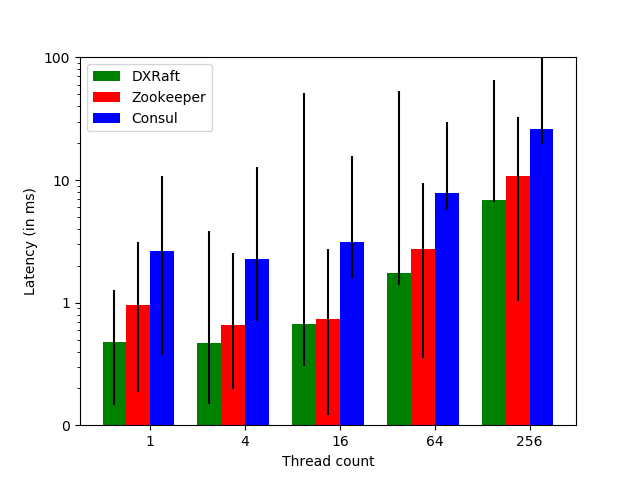
\includegraphics[width=\textwidth]{img/latency.png}
		\caption{100\% Writes.}
	\end{subfigure}
	\begin{subfigure}[t]{0.45\textwidth}
		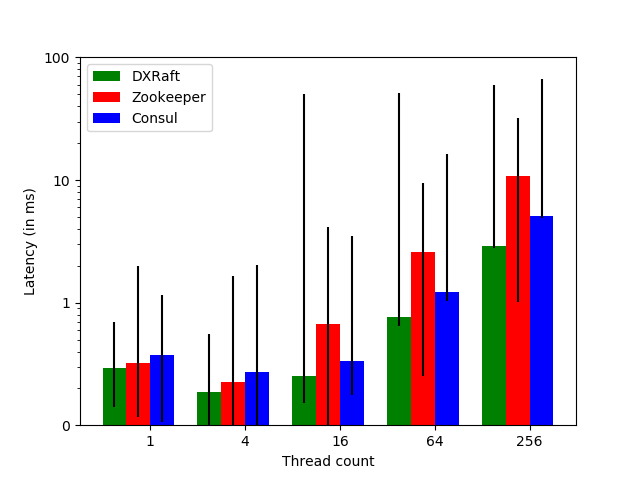
\includegraphics[width=\textwidth]{img/latency2.png}
		\caption{25\% Writes, 75\% Reads.}
	\end{subfigure}
	\caption{Latenzen der Systeme. Der Benchmark wurde mit einem Client und drei Server durchgeführt.}
	\label{fig:latency}
\end{figure}

Die Abbildung \ref{fig:latency} zeigt die Latenz der verschiedenen Systeme bei zunehmender Anzahl an Client-Threads. Die Client-Threads wurden auf einem Client ausgeführt und sendeten die Anfragen blockierend an die Systeme. Jeder Client-Thread sendete also nur eine Anfrage gleichzeitig. Die Systeme bestanden jeweils aus drei Servern, die am Konsensus-Algorithmus teilnahmen. Die farbigen Balken zeigen dabei die durchschnittliche Latenz, während die schwarzen Striche den Bereich des 99,9ten Perzentils zeigen. Es wurden zwei Workloads getestet: Ein Workload mit 100 \% Writes zeigt die Performance der Konsensus-Implementierung, da dabei alle Anfragen von allen Servern in der gleichen Reihenfolge bearbeitet werden müssen. Ein Workload mit nur 25\% Writes und 75\% Reads entspricht mehr einem realen Workload. Da Zookeeper keine Leseanfragen mit strikter Konsistenz anbietet, wurden die Leseanfragen mit abgeschwächter Konsistenz ausgeführt: Bei DXRaft wird der ebenfalls keine strikte Konsistenz gefordert und bei Consul wird der Konsistenzmodus \textit{stale} verwendet. Bei Lesanfragen mit strikter Konsistenz würden die Ergebnisse vermutlich stark den Ergebnissen des Workloads mit aussschließlich Schreibanfragen ähneln, da diese dann ebenfalls den Konsensus-Algorithmus durchlaufen müssen.

Insgesamt ist die durchschnittliche Latenz bei DXRaft am geringsten. Die anderen Systeme scheinen also etwas mehr Arbeit pro Anfrage zu verrichten. Möglicherweise könnte dies an fehlenden Features in DXRaft liegen, wie z.B. eine Log-Kompaktierung, die nebenläufige Arbeit erfordert. Dennoch scheint DXRaft im Vergleich mit den anderen Systemen im Durschnitt gute Latenzen zu haben. 

Im 99,9ten Perzentil nimmt dagegen bei DXRaft die maximale Latenz im Vergleich zum Durchschnitt mit steigender Anzahl an Anfragen deutlich zu. Dies lässt sich bei den anderen Systemen nicht beobachten. Die Latenzen von DXRaft sind also deutlich weniger stabil als die Latenzen bei den anderen Systemen. Hier könnte DXRaft eventuell durch mehr Parallelität und bessere Messaging-Implementierung stabiler werden, z.B. durch das gleichzeitige Versenden mehrerer \textit{Append Entries}-Request des Leaders an die Follower. Auch das Minimum im 99,9ten Perzentil nähert sich bei DXRaft mit steigender Anzahl an Anfragen immer mehr dem Durchschnitt. Dies lässt sich bei Consul ebenso beobachten. Bei Zookeeper ist dagegen ist auch das Minimum im Vergleich zum Durchschnitt sehr stabil.

Bei bis zu 16 Threads steigen die Latenzen nicht stark an. Bei Consul und Zookeeper nehmen die Latenzen sogar zunächst im Vergleich zu einem einzelnen Thread ab. Dies könnte durch eine Bearbeitung in Batches und durch höhere Parallelität hervorgerufen werden. Bei DXRaft ist jedoch keine Abnahme der Latenz von Schreibanfragen zu erkennen. Möglicherweise könnte hier durch mehr Parallelität ebenfalls die Latenz verringert werden, z.B. durch mehrere Message-Handler-Threads und feingranulare Sperren.

Bei dem Workload mit 75\% Reads sind die Latenzen insgesamt erwartungsgemäß niedriger. Ansonsten ändert sich wenig: DXRaft hat weiterhin die geringsten durchschnittlichen Latenzen, jedoch sind diese weniger stabil. Ein Unterschied ist jedoch, dass Zookeeper bei diesem Workload ab 16 Threads eine schlechtere durchschnittliche Latenz hat im Vergleich zu Consul. Zookeeper benötigt also für die Leseanfragen im Vergleich mit den anderen Systemen mehr Zeit, während sich bei Consul der Unterschied zu DXRaft verringert. Consul scheint die Leseanfragen also zumindest im Konsistenzmodus \textit{stale} sehr schnell bearbeiten zu können.

\section{Durchsatz}

Abbildung \ref{fig:throughput} zeigt den Durchsatz der Systeme bei in \ref{latency} beschriebenem Benchmark. Dies entspricht in etwa den Ergebnissen des Vergleichs der Latenzen: DXRaft hat den höchsten Durchsatz, bei Schreibanfragen hat Zookeeper den zweithöchsten Durchsatz und mit Leseanfragen hat Consul den zweithöchsten Durchsatz.

Interessant ist hierbei, dass der maximale Durchsatz bei Zookeeper bereits bei 16 Threads erreicht zu sein scheint, da er bei mehr Threads nicht mehr steigt. Bei DXRaft steigt der Durchsatz dagegen noch bis 64 Threads. Beim Workload mit Leseanfragen steigt der Durchsatz sogar bis 256 Threads. Dies könnte bei Leseanfragen durch eine bessere Verteilung der Anfragen auf die Server zustande kommen. Da die Leseanfragen nicht strikt konsistent sein müssen, können diese von jedem Server im Cluster bearbeitet werden. In DXRaft wird deswegen im Client ein zufälliger Server gewählt, an den die Anfrage geschickt wird. Da der Durchsatz bei Consul und Zookeeper mit Leseanfragen ab 16 Threads nicht mehr steigt, scheinen die Anfragen nicht gut auf alle Server verteilt werden.

\begin{figure}[t]
	\centering
	\begin{subfigure}[t]{0.45\textwidth}
		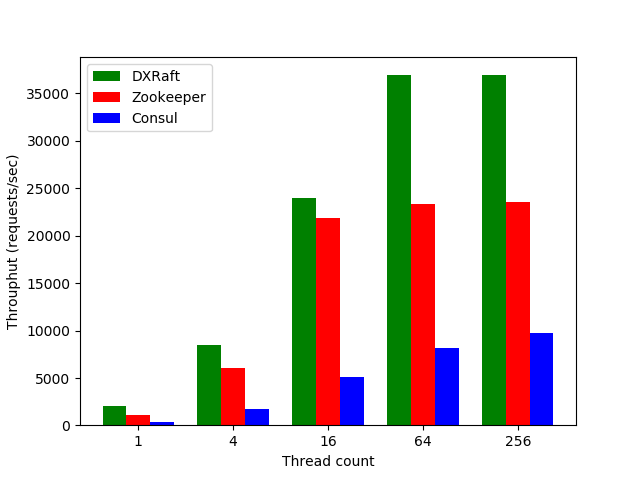
\includegraphics[width=\textwidth]{img/throughput.png}
		\caption{100\% Writes.}
	\end{subfigure}
	\begin{subfigure}[t]{0.45\textwidth}
		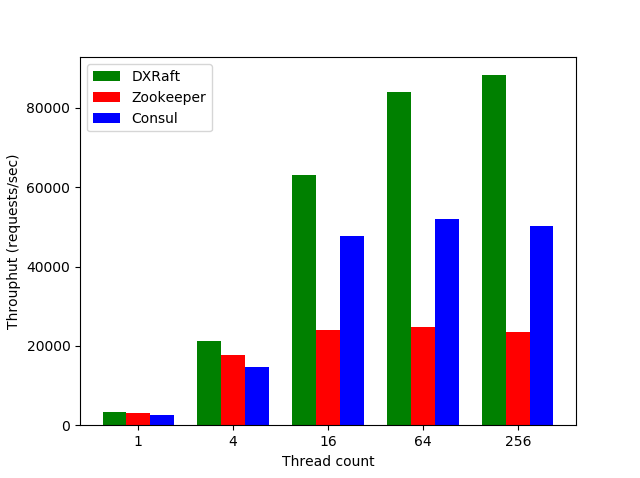
\includegraphics[width=\textwidth]{img/throughput2.png}
		\caption{25\% Writes, 75\% Reads.}
	\end{subfigure}
	\caption{Durchsatz der Systeme. Der Benchmark wurde mit einem Client und drei Server durchgeführt.}
	\label{fig:throughput}
\end{figure}


\section{Latenz in DXRaft}
\label{dxraft-latency}

Um das Optimierungspotenzial von DXRaft zu bestimmen, kann die Aufteilung der Latenz der Anfragen ermittelt werden. Dabei kann die Bearbeitung einer (Schreib-)Anfrage in folgende Aktionen aufgeteilt:
\begin{itemize}
	\item \textbf{Kommunikation zwischen Client und Leader}: Zeit, den die Kommunikation von Client und Leader benötigt, also Senden der Anfrage, erhalten der Anfrage, senden der Antwort und erhalten der Antwort. Diese wird ermittelt, indem von der beim Client ermittelten gesamten Laufzeit der Anfrage die Zeit für die Leader-Aktionen abgezogen wird.
	\item \textbf{Anhängen an das Log des Leaders}: Um eine Schreibanfrage auszuführen, muss der Leader einen Log-Eintrag erstellen und diesen an sein Log anhängen. Da das Log auf Festplatte persistiert werden muss, schließt dies einen Schreibzugriff auf die Festplatte mit ein und ist deswegen interessant.
	\item \textbf{Konsensus}: Zeit, um den Log-Eintrag auf eine Mehrheit der Follower zu replizieren. Dies schließt also die Kommunikation mit einer Mehrheit der Follower und die Verarbeitung des Eintrags bei den Followern ein. Dabei muss der Log-Eintrag auch vom Follower an sein Log angehängt werden, sodass dieser ebenfalls auf die Festplatte schreiben muss.
\end{itemize}

Interessant sind vor allem die Schreibanfragen, da diese durch den Konsensus-Algorithmus laufen müssen und dadurch länger benötigen als Leseanfragen. Abbildung \ref{fig:latency-analysis} visualisiert, welche Aktionen wie viel Zeit benötigen. Die Daten wurden mit einem Cluster aus drei DXRaft-Servern und einem Client mit vier Threads ermittelt. \\

In \ref{fig:request-avg} ist die durchschnittliche Dauer der beschriebenen Aktionen dargestellt. Im Durchschnitt lässt sich vor allem erkennen, dass die Zeit für das Anhängen an das Log sehr kurz ist und somit keinen Flaschenhals darstellt, obwohl dabei auf die Festplatte geschrieben werden muss. Die größte Zeit geht offensichtlich bei der Kommunikation verloren, etwa in gleichem Maße zwischen Client und Leader und zwischen Leader und Follower. Wenn die durchschnittliche Latenz noch verbessert werden sollte, könnte man also bei beiden Kommunikationen ansetzen. \\

In \ref{fig:request-max} ist die maximale Dauer der Aktionen dargestellt. Dabei ist festzustellen, dass auch die maximale Dauer der Kommunikation zwischen Client und Leader und zwischen Leader und Follower ähnlich groß ist. Insgesamt ist das Maximum mit etwa 40-50 ms bei beiden Kommunikationsaktionen sehr groß, insbesondere im Vergleich zum Durchschnitt. Es sollte mit den beschriebenen Optimierungsmöglichkeiten, z.B. mehr Parallelisierung bei der Verarbeitung von Nachrichten, möglich sein, das Maximum zu senken. Möglicherweise könnte auch der Garbage Collector dafür sorgen, dass die Nachrichtenverarbeitung unterschiedlich lange benötigt. Hier könnte mit anderen Garbage Collectoren experimentiert werden, die möglichst wenige Pausen der Anwendung verursachen.

Interessant ist auch die Verteilung bei der Anfrage, die die längste Zeit benötigt hat. Diese ist in \ref{fig:request-longest} zu sehen. Dabei ist auffällig, dass bei der längsten Anfrage die Zeit fast ausschließlich bei der Kommunikation zwischen Client und Leader verloren gegangen ist. Um das Maximum zu senken, sollte also zunächst diese Kommunikation betrachtet werden. Hier könnte möglicherweise der Session-Mechanismus Auslöser sein, da das Leeren der Session eine zusätzliche Anfrage benötigt (siehe \ref{sessions} für eine Beschreibung des Session-Mechanismus). Die Zeit für diese Anfrage fällt ebenfalls in die Kommunikation zwischen Client und Leader, da die Zeiten nur für die eigentliche Anfrage gemessen wurden.

\begin{figure}[t]
	\centering
	\begin{subfigure}[t]{1\textwidth}
		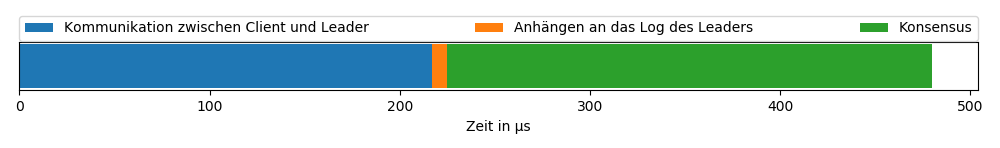
\includegraphics[width=\textwidth]{img/request_avg_timing.png}
		\caption{Durchschnittliche Anfrage.}
		\label{fig:request-avg}
	\end{subfigure}
	\begin{subfigure}[t]{1\textwidth}
		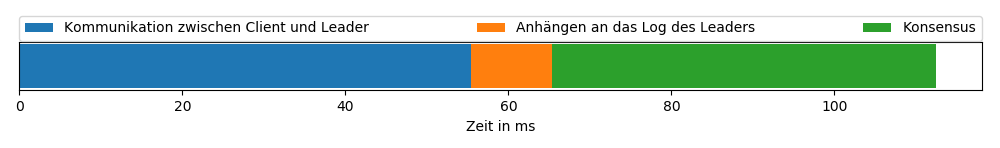
\includegraphics[width=\textwidth]{img/request_max_timing.png}
		\caption{Maximale Zeiten.}
		\label{fig:request-max}
	\end{subfigure}
	\begin{subfigure}[t]{1\textwidth}
		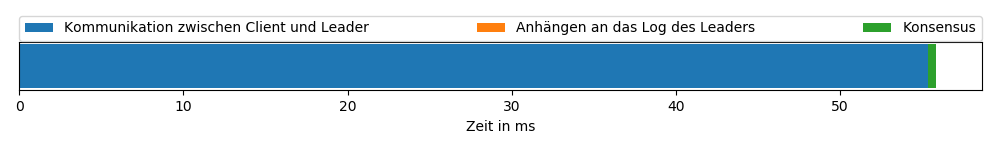
\includegraphics[width=\textwidth]{img/request_longest_timing.png}
		\caption{Längste Anfrage.}
		\label{fig:request-longest}
	\end{subfigure}
 	\caption{Aufteilung der Latenz in DXRaft.}
 	\label{fig:latency-analysis}
\end{figure}

\section{Leader Election}

Für die Bewertung des Systems ist nicht nur die Performance unter optimalen Bedingungen wichtig, sondern auch die Toleranz von Ausfällen. Dies ist gerade die Motivation für die Entwicklung des Systems. Leider ist es schwierig, eine Netzwerkpartitionierung zu simulieren. Eine Ausfall eines oder mehrere lässt sich dagegen einfacher hervorrufen. Der Ausfall eines Followers ist weniger interessant als der eines Leaders, da sich der Ablauf der Anfrageverarbeitung beim Ausfall eines Followers kaum ändert. Bei dem Ausfall des Leaders muss dagegen das Cluster den Ausfall erkennen, einen neuen Leader bestimmen und die Anfragen müssen zum neuen Leader geleitet werden. \\
Abbildung \ref{fig:leader-crash} zeigt die Entwicklung der durchschnittlichen und maximalen Latenz mit der Zeit. Die Daten wurden wieder mit dem gleichen Benchmark wie zuvor ermittelt, mit drei Servern und einem Client mit vier Threads. Dabei wurde jeweils während der Laufzeit der Leader-Prozess zum Absturz gebracht. Dies geschah etwa zwischen Sekunde 20 und 30. \\
Die Clients von Zookeeper und Consul werfen bei einem Verbindungsabbruch zum Leader eine Exception, die die Anwendung davon benachrichtigt. Diese wurden ignoriert und die Anfragen wurden sofort erneut gesendet, um möglichst schnell eine Antwort zu erhalten. Das finden des neuen Leaders wird jedoch von den Clients automatisch übernommen. Bei DXRaft wird das erneute Senden der Anfragen bereits automatisch vom Client übernommen, solange eine bestimmte Zeit nicht überschritten wird. \\
Auf der Abbildung ist jeweils der Zeitpunkt des Leader-Ausfalls klar zu erkennen. Da der Durchschnitt und das Maximum über den Zeitraum von einer Sekunde bestimmt wurde, ist bei Zookeeper und Consul eine Lücke im Graphen, die aussagt, dass in dieser Sekunde keine Anfrage verarbeitet wurde. Es ist festzustellen, dass es nach dem Ausfall des Leaders bei DXRaft nur etwa eine Sekunde dauert, bis Anfragen wieder verarbeitet werden können. Bei Zookeeper dauert dies etwas länger, etwa 2-3 Sekunden. Bei Consul werden sogar über 10 Sekunden keine Anfragen beantwortet. Diese Ausfallerkennung oder die Leader Election scheint bei Consul also sehr viel Zeit zu benötigen, obwohl Consul ebenso wie DXRaft Raft als Algorithmus nutzt. DXRaft scheint den Ausfall des Leaders dagegen, auch im Vergleich mit den anderen Systemen, sehr schnell kompensieren zu können.

\begin{figure}[t]
	\centering
	\begin{subfigure}[t]{0.45\textwidth}
		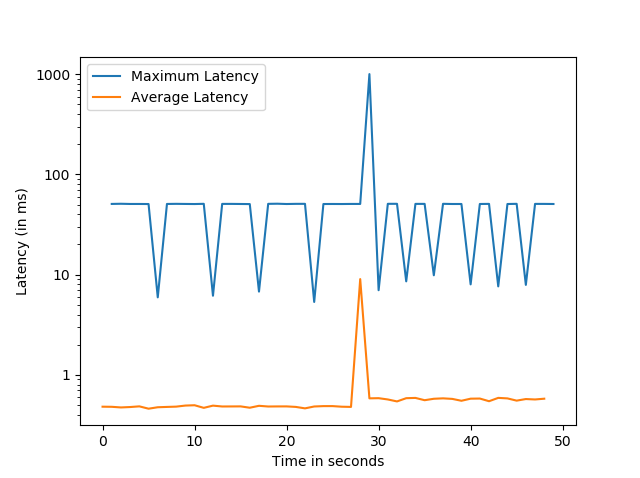
\includegraphics[width=\textwidth]{img/leader_crash_dxraft.png}
		\caption{DXRaft.}
	\end{subfigure}
	\begin{subfigure}[t]{0.45\textwidth}
		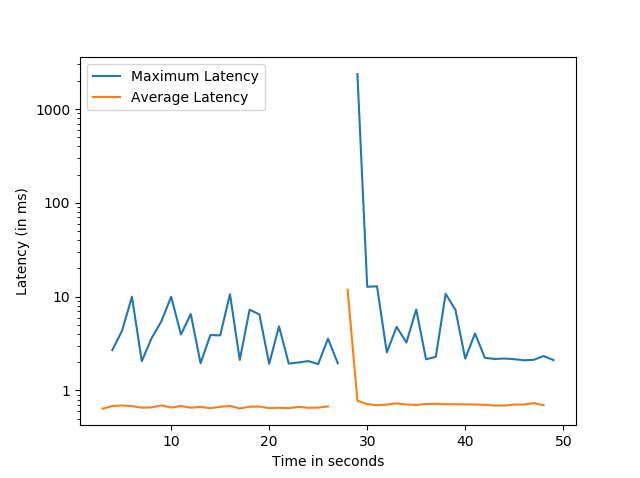
\includegraphics[width=\textwidth]{img/leader_crash_zk.png}
		\caption{Zookeeper.}
	\end{subfigure}
	\begin{subfigure}[t]{0.45\textwidth}
		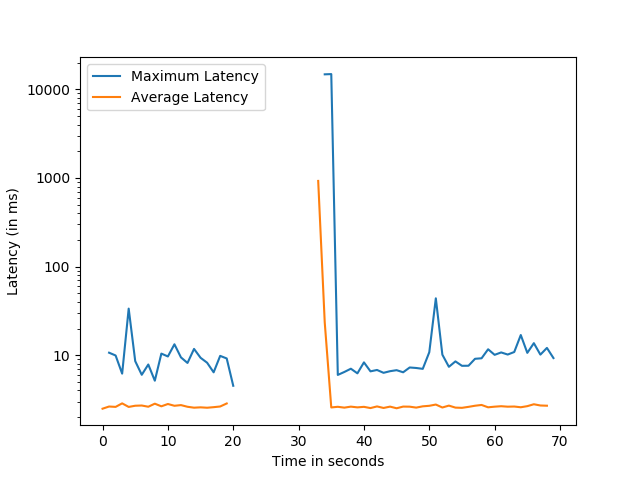
\includegraphics[width=\textwidth]{img/leader_crash_consul.png}
		\caption{Consul.}
	\end{subfigure}
	\caption{Latenz bei einem Leader-Crash.}
	\label{fig:leader-crash}
\end{figure}


\chapter{Fazit}

In dieser Arbeit wurde ein verteilter Koordinierungsdienst namens DXRaft entwickelt und implementiert. Dafür wurden zunächst die Anforderungen an das System formuliert. Dann wurde analysiert, wie ein solches System implementiert werden kann. Dabei wurde festgestellt, dass für die formulierten Anforderungen ein Einigungsalgorithmus implementiert werden muss. Deshalb wurden verschiedene Einigungsalgorithmen vorgestellt und analysiert. Dabei wurde Raft als zu implementierender Algorithmus ausgewählt. \\
Es wurden die Probleme und die Lösungen bei der Implementierung erläutert. Dabei wurde das Konzept der Implementierung erläutert. Es wurde erklärt, wie das System Nachrichten austauscht und wie das Bootstrapping abläuft. Außerdem wurde ein Session-Mechanismus und eine Möglichkeit der Änderung der Clusterkonfiguration während des laufenden Betriebs implementiert. Desweiteren wurde erklärt, wie das System das Log effizient auf der Festplatte persistiert und wie die Schnittstelle des Clients aufgebaut ist. Schließlich wurde erläutert, wie durch Tests sichergestellt wurde, dass das System korrekt funktioniert. \\
 Dann wurde das System evaluiert, in dem es mit anderen ähnlichen in der Industrie verwendeten Systemen verglichen wurde. Dabei wurde festgestellt, dass das implementierte System bei der durchschnittlichen Latenz und beim Durchsatz etwas bessere Ergebniss liefert als die anderen Systeme. Auch den Ausfall eines Leaders kann das System im Vergleich zu den anderen System gut kompensieren und wählt sehr schnell einen neuen Leader um mit dem Bearbeiten von Anfragen fortzufahren. Jedoch ist die Latenz nicht so stabil wie bei den anderen Systemen, da die maximale Latenz höher ist. Deshalb wurde noch untersucht, wie die Latenz in DXRaft zustande kommt. Dabei wurde festgestellt, dass vor allem die Kommunikation die Höhe der Latenz bedingt. Es wurde sowohl die Kommunikation zwischen Client und Server als auch die Kommunikation zwischen der Servern als Engpässe identifiziert. \\
Schließlich wurden Verbesserungsmöglichkeiten für weitere Arbeiten aufgezeigt. Diese umfassen eine Log-Kompaktierung, das Recovery von ausgefallenen Servern, das Testen auf \textit{Linearizability} und Performanceverbesserungen durch Optimierung der Thread-Architektur und des Nachrichtenaustausches.\\

\end{abschlussarbeit}
\end{document}

